\documentclass{article}

% if you need to pass options to natbib, use, e.g.:
% \PassOptionsToPackage{numbers, compress}{natbib}
% before loading neurips_2023

\usepackage[preprint]{neurips_2023}

% to compile a preprint version, e.g., for submission to arXiv, add add the
% [preprint] option:
% \usepackage[preprint]{neurips_2023}

% to compile a camera-ready version, add the [final] option, e.g.:
% \usepackage[final]{neurips_2023}

% to avoid loading the natbib package, add option nonatbib:
% \usepackage[nonatbib]{neurips_2023}

% TOC for document parts, must be included before hyperref!
% (https://latex.org/forum/viewtopic.php?t=2014)
\usepackage{titletoc}
%%% Local Variables:
%%% mode: latex
%%% TeX-master: "../main"
%%% End:

\usepackage[utf8]{inputenc} % allow utf-8 input
\usepackage[T1]{fontenc}    % use 8-bit T1 fonts
\usepackage{hyperref}       % hyperlinks
\usepackage{url}            % simple URL typesetting
\usepackage{booktabs}       % professional-quality tables
\usepackage{amsfonts}       % blackboard math symbols
\usepackage{nicefrac}       % compact symbols for 1/2, etc.
\usepackage{microtype}      % microtypography
\usepackage{xcolor}         % colors
%%% Local Variables:
%%% mode: latex
%%% TeX-master: "../main"
%%% End:

% requirements
\usepackage{amsmath}
\usepackage{amssymb}
\usepackage{bm}
\usepackage{mathtools}

% Random variables
\def\reta{{\textnormal{$\eta$}}}
\def\ra{{\textnormal{a}}}
\def\rb{{\textnormal{b}}}
\def\rc{{\textnormal{c}}}
\def\rd{{\textnormal{d}}}
\def\re{{\textnormal{e}}}
\def\rf{{\textnormal{f}}}
\def\rg{{\textnormal{g}}}
\def\rh{{\textnormal{h}}}
\def\ri{{\textnormal{i}}}
\def\rj{{\textnormal{j}}}
\def\rk{{\textnormal{k}}}
\def\rl{{\textnormal{l}}}
% rm is already a command, just don't name any random variables m
\def\rn{{\textnormal{n}}}
\def\ro{{\textnormal{o}}}
\def\rp{{\textnormal{p}}}
\def\rq{{\textnormal{q}}}
\def\rr{{\textnormal{r}}}
\def\rs{{\textnormal{s}}}
\def\rt{{\textnormal{t}}}
\def\ru{{\textnormal{u}}}
\def\rv{{\textnormal{v}}}
\def\rw{{\textnormal{w}}}
\def\rx{{\textnormal{x}}}
\def\ry{{\textnormal{y}}}
\def\rz{{\textnormal{z}}}

% Random vectors
\def\rvepsilon{{\mathbf{\epsilon}}}
\def\rvtheta{{\mathbf{\theta}}}
\def\rva{{\mathbf{a}}}
\def\rvb{{\mathbf{b}}}
\def\rvc{{\mathbf{c}}}
\def\rvd{{\mathbf{d}}}
\def\rve{{\mathbf{e}}}
\def\rvf{{\mathbf{f}}}
\def\rvg{{\mathbf{g}}}
\def\rvh{{\mathbf{h}}}
\def\rvu{{\mathbf{i}}}
\def\rvj{{\mathbf{j}}}
\def\rvk{{\mathbf{k}}}
\def\rvl{{\mathbf{l}}}
\def\rvm{{\mathbf{m}}}
\def\rvn{{\mathbf{n}}}
\def\rvo{{\mathbf{o}}}
\def\rvp{{\mathbf{p}}}
\def\rvq{{\mathbf{q}}}
\def\rvr{{\mathbf{r}}}
\def\rvs{{\mathbf{s}}}
\def\rvt{{\mathbf{t}}}
\def\rvu{{\mathbf{u}}}
\def\rvv{{\mathbf{v}}}
\def\rvw{{\mathbf{w}}}
\def\rvx{{\mathbf{x}}}
\def\rvy{{\mathbf{y}}}
\def\rvz{{\mathbf{z}}}

% Elements of random vectors
\def\erva{{\textnormal{a}}}
\def\ervb{{\textnormal{b}}}
\def\ervc{{\textnormal{c}}}
\def\ervd{{\textnormal{d}}}
\def\erve{{\textnormal{e}}}
\def\ervf{{\textnormal{f}}}
\def\ervg{{\textnormal{g}}}
\def\ervh{{\textnormal{h}}}
\def\ervi{{\textnormal{i}}}
\def\ervj{{\textnormal{j}}}
\def\ervk{{\textnormal{k}}}
\def\ervl{{\textnormal{l}}}
\def\ervm{{\textnormal{m}}}
\def\ervn{{\textnormal{n}}}
\def\ervo{{\textnormal{o}}}
\def\ervp{{\textnormal{p}}}
\def\ervq{{\textnormal{q}}}
\def\ervr{{\textnormal{r}}}
\def\ervs{{\textnormal{s}}}
\def\ervt{{\textnormal{t}}}
\def\ervu{{\textnormal{u}}}
\def\ervv{{\textnormal{v}}}
\def\ervw{{\textnormal{w}}}
\def\ervx{{\textnormal{x}}}
\def\ervy{{\textnormal{y}}}
\def\ervz{{\textnormal{z}}}

% Random matrices
\def\rmA{{\mathbf{A}}}
\def\rmB{{\mathbf{B}}}
\def\rmC{{\mathbf{C}}}
\def\rmD{{\mathbf{D}}}
\def\rmE{{\mathbf{E}}}
\def\rmF{{\mathbf{F}}}
\def\rmG{{\mathbf{G}}}
\def\rmH{{\mathbf{H}}}
\def\rmI{{\mathbf{I}}}
\def\rmJ{{\mathbf{J}}}
\def\rmK{{\mathbf{K}}}
\def\rmL{{\mathbf{L}}}
\def\rmM{{\mathbf{M}}}
\def\rmN{{\mathbf{N}}}
\def\rmO{{\mathbf{O}}}
\def\rmP{{\mathbf{P}}}
\def\rmQ{{\mathbf{Q}}}
\def\rmR{{\mathbf{R}}}
\def\rmS{{\mathbf{S}}}
\def\rmT{{\mathbf{T}}}
\def\rmU{{\mathbf{U}}}
\def\rmV{{\mathbf{V}}}
\def\rmW{{\mathbf{W}}}
\def\rmX{{\mathbf{X}}}
\def\rmY{{\mathbf{Y}}}
\def\rmZ{{\mathbf{Z}}}

% Elements of random matrices
\def\ermA{{\textnormal{A}}}
\def\ermB{{\textnormal{B}}}
\def\ermC{{\textnormal{C}}}
\def\ermD{{\textnormal{D}}}
\def\ermE{{\textnormal{E}}}
\def\ermF{{\textnormal{F}}}
\def\ermG{{\textnormal{G}}}
\def\ermH{{\textnormal{H}}}
\def\ermI{{\textnormal{I}}}
\def\ermJ{{\textnormal{J}}}
\def\ermK{{\textnormal{K}}}
\def\ermL{{\textnormal{L}}}
\def\ermM{{\textnormal{M}}}
\def\ermN{{\textnormal{N}}}
\def\ermO{{\textnormal{O}}}
\def\ermP{{\textnormal{P}}}
\def\ermQ{{\textnormal{Q}}}
\def\ermR{{\textnormal{R}}}
\def\ermS{{\textnormal{S}}}
\def\ermT{{\textnormal{T}}}
\def\ermU{{\textnormal{U}}}
\def\ermV{{\textnormal{V}}}
\def\ermW{{\textnormal{W}}}
\def\ermX{{\textnormal{X}}}
\def\ermY{{\textnormal{Y}}}
\def\ermZ{{\textnormal{Z}}}

% Vectors
\def\vzero{{\bm{0}}}
\def\vone{{\bm{1}}}
\def\vmu{{\bm{\mu}}}
\def\vnu{{\bm{\nu}}}
\def\vtheta{{\bm{\theta}}}
\def\vepsilon{{\bm{\epsilon}}}
\def\vgamma{{\bm{\gamma}}}
\def\vdelta{{\bm{\delta}}}
\def\vDelta{{\bm{\Delta}}}
\def\va{{\bm{a}}}
\def\vb{{\bm{b}}}
\def\vc{{\bm{c}}}
\def\vd{{\bm{d}}}
\def\ve{{\bm{e}}}
\def\vetilde{\bm{\tilde{e}}}
\def\vell{{\bm{\ell}}}
\def\vf{{\bm{f}}}
\def\vg{{\bm{g}}}
\def\vh{{\bm{h}}}
\def\vi{{\bm{i}}}
\def\vj{{\bm{j}}}
\def\vk{{\bm{k}}}
\def\vl{{\bm{l}}}
\def\vm{{\bm{m}}}
\def\vmhat{{\bm{\hat{m}}}}
\def\vn{{\bm{n}}}
\def\vo{{\bm{o}}}
\def\vp{{\bm{p}}}
\def\vphi{{\bm{\phi}}}
\def\vq{{\bm{q}}}
\def\vr{{\bm{r}}}
\def\vs{{\bm{s}}}
\def\vstilde{\bm{\tilde{s}}}
\def\vt{{\bm{t}}}
\def\vu{{\bm{u}}}
\def\vv{{\bm{v}}}
\def\vvhat{{\bm{\hat{v}}}}
\def\vw{{\bm{w}}}
\def\vx{{\bm{x}}}
\def\vy{{\bm{y}}}
\def\vytilde{{\bm{\tilde{y}}}}
\def\vyhat{{\bm{\hat{y}}}}
\def\vz{{\bm{z}}}

% Elements of vectors
\def\evalpha{{\alpha}}
\def\evbeta{{\beta}}
\def\evepsilon{{\epsilon}}
\def\evlambda{{\lambda}}
\def\evomega{{\omega}}
\def\evmu{{\mu}}
\def\evpsi{{\psi}}
\def\evsigma{{\sigma}}
\def\evtheta{{\theta}}
\def\eva{{a}}
\def\evb{{b}}
\def\evc{{c}}
\def\evd{{d}}
\def\eve{{e}}
\def\evf{{f}}
\def\evg{{g}}
\def\evh{{h}}
\def\evi{{i}}
\def\evj{{j}}
\def\evk{{k}}
\def\evl{{l}}
\def\evm{{m}}
\def\evn{{n}}
\def\evo{{o}}
\def\evp{{p}}
\def\evq{{q}}
\def\evr{{r}}
\def\evs{{s}}
\def\evt{{t}}
\def\evu{{u}}
\def\evv{{v}}
\def\evw{{w}}
\def\evx{{x}}
\def\evy{{y}}
\def\evyhat{{\hat{y}}}
\def\evz{{z}}

% Matrix
\def\mA{{\bm{A}}}
\def\mB{{\bm{B}}}
\def\mC{{\bm{C}}}
\def\mD{{\bm{D}}}
\def\mE{{\bm{E}}}
\def\mF{{\bm{F}}}
\def\mG{{\bm{G}}}
\def\mGtilde{\bm{\tilde{G}}}
\def\mH{{\bm{H}}}
\def\mI{{\bm{I}}}
\def\mJ{{\bm{J}}}
\def\mK{{\bm{K}}}
\def\mL{{\bm{L}}}
\def\mM{{\bm{M}}}
\def\mN{{\bm{N}}}
\def\mO{{\bm{O}}}
\def\mP{{\bm{P}}}
\def\mQ{{\bm{Q}}}
\def\mR{{\bm{R}}}
\def\mS{{\bm{S}}}
\def\mT{{\bm{T}}}
\def\mU{{\bm{U}}}
\def\mV{{\bm{V}}}
\def\mW{{\bm{W}}}
\def\mX{{\bm{X}}}
\def\mY{{\bm{Y}}}
\def\mZ{{\bm{Z}}}
\def\mBeta{{\bm{\beta}}}
\def\mGamma{{\bm{\Gamma}}}
\def\mPhi{{\bm{\Phi}}}
\def\mPi{{\bm{\Pi}}}
\def\mLambda{{\bm{\Lambda}}}
\def\mSigma{{\bm{\Sigma}}}
\def\mOmega{{\bm{\Omega}}}
\def\mStilde{\bm{\tilde{\mS}}}
\def\mGtilde{\bm{\tilde{\mG}}}
\def\mGoverline{{\bm{\overline{G}}}}

% Tensor
\DeclareMathAlphabet{\mathsfit}{\encodingdefault}{\sfdefault}{m}{sl}
\SetMathAlphabet{\mathsfit}{bold}{\encodingdefault}{\sfdefault}{bx}{n}
\newcommand{\tens}[1]{\bm{\mathsfit{#1}}}
\def\tA{{\tens{A}}}
\def\tB{{\tens{B}}}
\def\tC{{\tens{C}}}
\def\tD{{\tens{D}}}
\def\tE{{\tens{E}}}
\def\tF{{\tens{F}}}
\def\tG{{\tens{G}}}
\def\tH{{\tens{H}}}
\def\tI{{\tens{I}}}
\def\tJ{{\tens{J}}}
\def\tK{{\tens{K}}}
\def\tL{{\tens{L}}}
\def\tM{{\tens{M}}}
\def\tN{{\tens{N}}}
\def\tO{{\tens{O}}}
\def\tP{{\tens{P}}}
\def\tPi{\bm{\mathsf{\Pi}}}
\def\tQ{{\tens{Q}}}
\def\tR{{\tens{R}}}
\def\tS{{\tens{S}}}
\def\tT{{\tens{T}}}
\def\tU{{\tens{U}}}
\def\tV{{\tens{V}}}
\def\tW{{\tens{W}}}
\def\tX{{\tens{X}}}
\def\tY{{\tens{Y}}}
\def\tZ{{\tens{Z}}}

% Graph
\def\gA{{\mathcal{A}}}
\def\gB{{\mathcal{B}}}
\def\gC{{\mathcal{C}}}
\def\gD{{\mathcal{D}}}
\def\gE{{\mathcal{E}}}
\def\gF{{\mathcal{F}}}
\def\gG{{\mathcal{G}}}
\def\gH{{\mathcal{H}}}
\def\gI{{\mathcal{I}}}
\def\gJ{{\mathcal{J}}}
\def\gK{{\mathcal{K}}}
\def\gL{{\mathcal{L}}}
\def\gM{{\mathcal{M}}}
\def\gN{{\mathcal{N}}}
\def\gO{{\mathcal{O}}}
\def\gP{{\mathcal{P}}}
\def\gQ{{\mathcal{Q}}}
\def\gR{{\mathcal{R}}}
\def\gS{{\mathcal{S}}}
\def\gT{{\mathcal{T}}}
\def\gU{{\mathcal{U}}}
\def\gV{{\mathcal{V}}}
\def\gW{{\mathcal{W}}}
\def\gX{{\mathcal{X}}}
\def\gY{{\mathcal{Y}}}
\def\gZ{{\mathcal{Z}}}

% Sets
\def\sA{{\mathbb{A}}}
\def\sB{{\mathbb{B}}}
\def\sC{{\mathbb{C}}}
\def\sD{{\mathbb{D}}}
% Don't use a set called E, because this would be the same as our symbol
% for expectation.
\def\sF{{\mathbb{F}}}
\def\sG{{\mathbb{G}}}
\def\sH{{\mathbb{H}}}
\def\sI{{\mathbb{I}}}
\def\sJ{{\mathbb{J}}}
\def\sK{{\mathbb{K}}}
\def\sL{{\mathbb{L}}}
\def\sM{{\mathbb{M}}}
\def\sN{{\mathbb{N}}}
\def\sO{{\mathbb{O}}}
\def\sP{{\mathbb{P}}}
\def\sQ{{\mathbb{Q}}}
\def\sR{{\mathbb{R}}}
\def\sS{{\mathbb{S}}}
\def\sT{{\mathbb{T}}}
\def\sU{{\mathbb{U}}}
\def\sV{{\mathbb{V}}}
\def\sW{{\mathbb{W}}}
\def\sX{{\mathbb{X}}}
\def\sY{{\mathbb{Y}}}
\def\sYhat{{\hat{\mathbb{Y}}}}
\def\sZ{{\mathbb{Z}}}
% Blackboard Greek characters: https://tex.stackexchange.com/a/3260
\DeclareSymbolFont{bbold}{U}{bbold}{m}{n}
\DeclareSymbolFontAlphabet{\mathbbold}{bbold}
\def\sTheta{{\mathbbold{\Theta}}}
\def\sOmega{{\mathbbold{\Omega}}}

% Entries of a matrix
\def\emLambda{{\Lambda}}
\def\emA{{A}}
\def\emB{{B}}
\def\emC{{C}}
\def\emD{{D}}
\def\emE{{E}}
\def\emF{{F}}
\def\emG{{G}}
\def\emH{{H}}
\def\emI{{I}}
\def\emJ{{J}}
\def\emK{{K}}
\def\emL{{L}}
\def\emM{{M}}
\def\emN{{N}}
\def\emO{{O}}
\def\emP{{P}}
\def\emQ{{Q}}
\def\emR{{R}}
\def\emS{{S}}
\def\emT{{T}}
\def\emU{{U}}
\def\emV{{V}}
\def\emW{{W}}
\def\emX{{X}}
\def\emY{{Y}}
\def\emZ{{Z}}
\def\emSigma{{\Sigma}}
\def\emPi{{\Pi}}

% entries of a tensor
% Same font as tensor, without \bm wrapper
\newcommand{\etens}[1]{\mathsfit{#1}}
\def\etLambda{{\etens{\Lambda}}}
\def\etA{{\etens{A}}}
\def\etB{{\etens{B}}}
\def\etC{{\etens{C}}}
\def\etD{{\etens{D}}}
\def\etE{{\etens{E}}}
\def\etF{{\etens{F}}}
\def\etG{{\etens{G}}}
\def\etH{{\etens{H}}}
\def\etI{{\etens{I}}}
\def\etJ{{\etens{J}}}
\def\etK{{\etens{K}}}
\def\etL{{\etens{L}}}
\def\etM{{\etens{M}}}
\def\etN{{\etens{N}}}
\def\etO{{\etens{O}}}
\def\etP{{\etens{P}}}
\def\etPi{\mathsf{\Pi}}
\def\etQ{{\etens{Q}}}
\def\etR{{\etens{R}}}
\def\etS{{\etens{S}}}
\def\etT{{\etens{T}}}
\def\etU{{\etens{U}}}
\def\etV{{\etens{V}}}
\def\etW{{\etens{W}}}
\def\etX{{\etens{X}}}
\def\etY{{\etens{Y}}}
\def\etZ{{\etens{Z}}}

% The true underlying data generating distribution
\newcommand{\pdata}{p_{\mathrm{data}}}
% The empirical distribution defined by the training set
\newcommand{\ptrain}{\hat{p}_{\mathrm{data}}}
\newcommand{\Ptrain}{\hat{P}_{\mathrm{data}}}
% The model distribution
\newcommand{\pmodel}{p_{\rm{model}}}
\newcommand{\Pmodel}{P_{\rm{model}}}
\newcommand{\ptildemodel}{\tilde{p}_{\rm{model}}}
% Stochastic autoencoder distributions
\newcommand{\pencode}{p_{\rm{encoder}}}
\newcommand{\pdecode}{p_{\rm{decoder}}}
\newcommand{\precons}{p_{\rm{reconstruct}}}

\newcommand{\laplace}{\mathrm{Laplace}} % Laplace distribution

\newcommand{\E}{\mathbb{E}}
\newcommand{\Ls}{\mathcal{L}}
\newcommand{\R}{\mathbb{R}}
\newcommand{\emp}{\tilde{p}}
\newcommand{\lr}{\alpha}
\newcommand{\reg}{\lambda}
\newcommand{\rect}{\mathrm{rectifier}}
\newcommand{\softmax}{\mathrm{softmax}}
\newcommand{\onehot}{\mathrm{onehot}}
\newcommand{\sigmoid}{\sigma}
\newcommand{\softplus}{\zeta}
\newcommand{\KL}{D_{\mathrm{KL}}}
\newcommand{\Var}{\mathrm{Var}}
\newcommand{\standarderror}{\mathrm{SE}}
\newcommand{\Cov}{\mathrm{Cov}}
% Wolfram Mathworld says $L^2$ is for function spaces and $\ell^2$ is for vectors
% But then they seem to use $L^2$ for vectors throughout the site, and so does
% wikipedia.
\newcommand{\normlzero}{L^0}
\newcommand{\normlone}{L^1}
\newcommand{\normltwo}{L^2}
\newcommand{\normlp}{L^p}
\newcommand{\normmax}{L^\infty}

\newcommand{\parents}{Pa} % See usage in notation.tex. Chosen to match Daphne's book.

\DeclareMathOperator*{\argmax}{arg\,max}
\DeclareMathOperator*{\argmin}{arg\,min}
\DeclareMathOperator*{\minimize}{minimize}
\DeclareMathOperator*{\maximize}{maximize}

\DeclareMathOperator{\sign}{sign}
\DeclareMathOperator{\mean}{mean}
\DeclareMathOperator{\vmap}{vmap}
\DeclareMathOperator{\reshape}{reshape}
\DeclareMathOperator{\Tr}{Tr}
\DeclareMathOperator{\diag}{diag}
\DeclareMathOperator{\eig}{eig}
\DeclareMathOperator{\rank}{rank}
\DeclareMathOperator{\vecspan}{span}
\DeclareMathOperator{\overlap}{overlap}
\DeclareMathOperator{\Cat}{Cat}

%%%%% NEW MATH DEFINITIONS %%%%%
\newcommand{\jac}{\mathrm{J}}
\newcommand{\grad}[1]{\ensuremath{\nabla_{\!{#1}}}}
\newcommand{\gradsquared}[1]{\ensuremath{\nabla_{\!{#1}}^{2}}}

% || for KLDivergence
\DeclarePairedDelimiterX{\KLdivx}[2]{(}{)}{%
  #1\;\delimsize\|\;#2%
}
\newcommand{\KLdiv}{\KL\KLdivx}

% | for a | b
\newcommand{\giventhat}[2]{#1\;|\;#2}

\let\ab\allowbreak
%%% Local Variables:
%%% mode: latex
%%% TeX-master: "../main"
%%% End:
 % follow DL notation from the Goodfellow book
% ===================================================================
% MATH
% ===================================================================
\usepackage{nicefrac} % fractions that fit into inline text

% ===================================================================
% REFERENCES
% ===================================================================
\usepackage{cleveref} % automatically adds type of reference, MUST BE LOADED AFTER AMSMATH

%%% Local Variables:
%%% mode: latex
%%% TeX-master: "../main"
%%% End:

\newcommand{\papertitle}{%
  A Kronecker-factored Approximate Gauß-Newton Method for Physics-Informed Neural Networks 
}
\title{\papertitle}

% The \author macro works with any number of authors. There are two commands
% used to separate the names and addresses of multiple authors: \And and \AND.
%
% Using \And between authors leaves it to LaTeX to determine where to break the
% lines. Using \AND forces a line break at that point. So, if LaTeX puts 3 of 4
% authors names on the first line, and the last on the second line, try using
% \AND instead of \And before the third author name.

\author{%
  Felix Dangel\thanks{Equal contribution, correspondence to \url{some mail}.}\\
  Vector Institute\\
  661 University Ave. \\
  Toronto, Canada \\
  \texttt{fdangel@vectorinstitute.ai} \\
  % examples of more authors
  \And
  Johannes M\"uller$^*$\\
  Department of Mathematics \\
  RWTH Aachen University \\
  Aachen, Germany \\
  \texttt{mueller@mathc.rwth-aachen.de} \\
  \And
  Marius Zeinhofer$^*$\\
  University Hospital \\
  University of Freiburg \\
  Freiburg, Germany \\
  \texttt{mariusz@simula.no} 
}
%%% Local Variables:
%%% mode: latex
%%% TeX-master: "../main"
%%% End:


\begin{document}

\maketitle

\begin{abstract}
  PINNs are hard to train with first-order methods.
  To train PINNs efficiently, we need to take into account the geometry implied by the PDE operator.
  Existing methods that consider this geometry compute and invert the full Gramian.
  However, these ENGD-based methods do not scale well to architectures with many parameters due to the quadratic memory and cubic time complexity of storing and inverting the Gramian.
  The challenge to develop approximations to the Gramian is that it requires taking the parameter derivative of the PDE operator, which itself contains higher-order derivative.
  Here, we propose a Kronecker factored approximation for the Gramian, which scales more favourably than existing approaches in terms of both time and memory, while showing similar performance downstream.
\end{abstract}

\section{Introduction}

PINNs are difficult to optimize.
\begin{itemize}
    \item PINNs receive ever growing amount of attention
    \item their failure to produce high accuracy solution when trained with variants of GD like Adam is well documented
    \item L-BFGS yields improved but still not very high accuracy
    \item Other suggestions: reweighting of the loss, specialized sampling strategies, greedy training, reformulation as saddle point problem
    \item recently, a variant of NG based on the geometry of the specific energy / PDE was proposed; yields greatly improved accuracy over direct gradient-based optimizers and enjoys the nice property that it can be shown to mimic Newton's method in function space; for PINNs it can be seen as Gau\ss-Newton method in the space of residuals, for other problems as a generalized GN?
    \item whereas, this method was shown to be able to produce highly accurate approximations of the solution of the PDE it comes with a considerable iteration cost as it involves the solution of a linear system of the size of the number of parameters. Hence, this is only feasible for networks of small to moderate size when done naively.
    \item we use the idea of KFAC and provide an efficient implementation; however, PDE terms appear in the Gramian, so existing implementations can not be used off the shelve 
\end{itemize}

\paragraph{Contribution:} \toodoo{Formulate our goal.}

\paragraph{Related work:}
\begin{itemize}
\item OG KFAC papers: \cite{martens2015optimizing}, \cite{martens2018kroneckerfactored}, double check similarities to RNNs
\item KFAC for Rayleigh quotients:
\item PINNs: recent preconditioning papers
\end{itemize}

%%% Local Variables:
%%% mode: latex
%%% TeX-master: "../main"
%%% End:


\section{Background}

\subsection{Physics informed neural networks (PINNs)}
%\begin{itemize}
%    \item PINNs are one of the most promising approaches to neural network based PDE solvers
%    \item
%\end{itemize}
Let us consider a domain $\Omega\subseteq\mathbb R^d$ and the Poisson equation %and how to write the Gramian/Fisher as the product of a Jacobian and its transpose, see equation \eqref{eq:Jacobian_Fischer}.
%Is this what you were after Felix?
%I think it differs from the standard setting in the sense that suddenly the Laplacian shows up.
%It can also be used to derive a matrix-free version of the energy natural gradient descent, like done in Hessian-free optimization.
%$\bullet$ We consider the Poisson equation
\begin{align*}\tag{PE}\label{eq:PE}
  -\Delta u & = f \quad \text{in }\Omega \\
  u & = g \quad \text{on }\partial\Omega
\end{align*}
where $f\in L^2(\Omega)$ and $g\in H^{3/2}(\partial\Omega)$ are some given right hand side and boundary values.
Here, $\Delta u = \sum_i \partial_{x_i}^2 u$ denotes the \emph{Laplacian} of the function $u$. 
Let us consider the function space energy 
  \[ E(u) = \frac{1}{2} \int_\Omega (\Delta u + f)^2 \mathrm dx + \frac12 \int_{\partial\Omega} (u-g)^2 \mathrm ds, \]
which is designed such that $u$ is a solution of~\eqref{eq:PE} if and only if $E(u)=0$. 
Hence, we discretize the integral and use the following loss function to train the parameters $\theta$ of a neural network
  %\[ L(\theta) \coloneqq E(u_\theta) = \frac{1}{2} \int_\Omega (\Delta u_\theta + f)^2 \mathrm dx + \frac12 \int_{\partial\Omega} (u_\theta-g)^2 \mathrm ds. \]
%Indeed, one can show that $L$ controls the error, i.e., $\lVert u_\theta - u^\star \rVert_{H^{1/2}(\Omega)} \le c_{\operatorname{reg}} \sqrt{L(\theta)}$, where $c_{\operatorname{reg}}$ denotes the regularity constant of the PDE, see~\cite{?}.
%In practice, we have to discretize the integrals in the PINN loss, and obtain the empirical loss function %with discretized integrals, is
\begin{align*}
  L(\theta)
  &=
    %\frac{1}{2N_\Omega} 
    L_\Omega(\theta) + %\frac{1}{2N_{\partial\Omega}}
    L_{\partial\Omega}(\theta)
  %\\&
  =
    \frac{1}{2N_\Omega} \sum_{i=1}^{N_\Omega} (\Delta u_\theta(x_i) + f(x_i))^2 + \frac{1}{2N_{\partial\Omega}}\sum_{i=1}^{N_{\partial\Omega}} ( u_\theta(x^b_i) - g(x^b_i))^2,
\end{align*}
where we denote by $(x_i)_{i=1,\dots,N_\Omega}$ the points in the interior of $\Omega$ and by $(x^b_i)_{i=1,\dots,N_{\partial\Omega}}$ the points on the boundary.
The number and choice of the points can be controlled by the practitioner, where different sampling strategies have been developed~\cite[text]{keylist}.

This approach is simple and intuitive and is usually associated with the possibility to work well for high-dimensional PDEs, however, it is well documented in the literature that it fails to produce satisfactory accuracy even for low-dimensional problems. 

\begin{itemize}
    \item If you run GD / Adam you get no good accuracy~\cite{?}
    \item L-BFGS improves things, but is not super satisfactory
    \item recently, function space inspired methods and preconditioners have been used with promising success~\cite[text]{CPINNs, ENG, preconditioning?, FS paper, Navier-Stokes}; we describe the approach we use here in more detail 
\end{itemize}

%%% Local Variables:
%%% mode: latex
%%% TeX-master: "../main"
%%% End:

\subsection{Energy natural gradients (ENGs)}

%\begin{itemize}
%    \item recently, energy NGs have been proposed
%    \item one can show that they mimic Newtons method in function space
%    \item yield very good accuracy
%    \item
%\end{itemize}

Natural gradients have been introduced by~\citet{amari1998natural} and have shown great success in reinforcement learning, and other problems...
The general idea is to replace the vanilla GD update rule by a preconditioned version
    \[ \vtheta_{k+1} = \vtheta_k - \eta_k \mG(\vtheta_k)^{-1} \nabla L(\vtheta_k), \]
where $\mG(\vtheta)\in\mathbb R^{p\times p}$, $\mG(\vtheta)_{ij} \coloneqq g_{u_\vtheta}(\partial_{\vtheta_i} u_\vtheta, \partial_{\vtheta_j} u_\vtheta)$ is a matrix capturing the function space geometry of the problem and its parametrization and $g$ denotes a suitable Riemannian metric. 
In least squares regression with data $(\vx_1, \vy_1), \dots, (\vx_N, \vy_N)$ the Gramian $\mG(\vtheta)$ is chosen as the (empirical) Fisher information matrix given by~\citep{martens2020new, eschenhagen2023kroneckerfactored} 
%\begin{equation}
%    F_I(\vtheta)_{ij} = \sum_{x} \frac{\partial_{\vtheta_i}p_\vtheta(x)\partial_{\vtheta_j}p_\vtheta(x)}{p_\vtheta(x)} = \sum_{x} \partial_{\vtheta_i} \log p_\vtheta(x) \partial_{\vtheta_j} \log p_\vtheta(x),
%\end{equation}
%in which case the Riemannian metric $g$ is given by the Fisher-Rao metric~\citet{}.
%For a supervised learning problem with training data $(\vx_1, \vy_1), \dots, (\vx_N, \vy_N)$ the (empirical) Fisher-information matrix commonly used, has entries the entries 
\begin{equation}
  %\mF(\vtheta)_{ij} = \sum_{n=1}^N \partial_{\vtheta_i} u_\vtheta(\vx_n)\partial_{\vtheta_j} u_\vtheta(\vx_n) \quad \text{maybe use?} 
  \mF(\vtheta) = \frac1N\sum_{n=1}^N \jac_{\vtheta} u_{\vtheta}(\vx_n)^\top \jac_{\vtheta} u_{\vtheta}(\vx_n)
  .
\end{equation}
To account for the PDE terms in the loss function in PINNs, 
%the models $u_\vtheta$ are functions rather than probability measures %$p_\vtheta$
%and the loss involves PDE terms.
%In order to adjust the definition of
%To capture the geometric properties of this specific problem we consider the following Fisher / Gramian matrix %to this problemThe energy natural gradient is for this example to use the Fischer/Gramian of the form
the Gramian matrix 
\begin{equation}
  \mG(\vtheta) = %\mG_\Omega(\vtheta) + \mG_{\partial\Omega}(\vtheta) =
  \underbrace{\frac1{{N_\Omega}} \sum_{n=1}^{N_\Omega} \jac_{\vtheta} \Delta u_\vtheta(\vx_n)^\top \jac_{\vtheta} \Delta u_\vtheta(\vx_n)}_{\eqqcolon \mG_\Omega(\vtheta)} + \underbrace{\frac1{{N_{\partial\Omega}}} \sum_{n=1}^{N_{\partial\Omega}} \jac_{\vtheta} u_\vtheta(\vx_n^b)^\top \jac_{\vtheta} u_\vtheta (\vx_n^b)}_{\eqqcolon \mG_{\partial\Omega}(\vtheta)}
  %\frac1{{N_\Omega}} \sum_{k=1}^{N_\Omega} \partial_{\vtheta_i} \Delta u_\vtheta(x_k) \partial_{\vtheta_j} \Delta u_\vtheta(x_k) + \frac1{{N_{\partial\Omega}}} \sum_{k=1}^{N_{\partial\Omega}} \partial_{\vtheta_i} u_\vtheta(x_k^b) \partial_{\vtheta_j} u_\vtheta (x_k^b)
\end{equation}
%where
%\begin{equation}\label{eq:FisherInterior}
%  F_\Omega(\vtheta)_{ij} = \frac1{{N_\Omega}} \sum_{k=1}^{N_\Omega} \partial_{\vtheta_i} \Delta u_\vtheta(x_k) \partial_{\vtheta_j} \Delta u_\vtheta(x_k)
  % = \frac1{{N_\Omega}} \sum_{i=1}^{N_\Omega} (\partial_{\vtheta_i} f_\vtheta) (\partial_{\vtheta_j} f_\vtheta ),
%\end{equation}
% where $f_\vtheta = \Delta u_\vtheta$.
%and
%\begin{equation}
%  F_{\partial\Omega}(\vtheta)_{ij} = \frac1{{N_{\partial\Omega}}} \sum_{k=1}^{N_{\partial\Omega}} \partial_{\vtheta_i} u_\vtheta(x_k^b) \partial_{\vtheta_j} u_\vtheta (x_k^b).
  % = \frac1{{N_\Omega}} \sum_{i=1}^{N_\Omega} (\partial_{\vtheta_i} f_\vtheta) (\partial_{\vtheta_j} f_\vtheta ),
%\end{equation}
has been suggested under the name \emph{energy natural gradient} (ENG), see~\cite{muller2023achieving}. 
The energy natural gradient method mimics Newton's method up to a projection onto the tangent space of the model and a discretization error that vanishes quadratically in the step size 
and improves the accuracy of PINNs by several orders of magnitude when compared to GD, Adam, or BFGS~\citep{muller2023achieving, ?}. 
The Gramian matrix $\mG(\theta)$ can be interpreted as the Gauß-Newton matrix of the residual function, see~\cite{} and Appendix....

%%% Local Variables:
%%% mode: latex
%%% TeX-master: "../main"
%%% End:

\subsection{Kronecker-factored Approximate Curvature (KFAC)}

\toodoo{F.D.
  Get to the point more quickly.
  Make notation throughout subsection consistent.}

KFAC was introduced by \citet{martens2015optimizing} to approximate the per-layer Fisher information matrix of a neural network's parameters for maximum likelihood estimation.
Assume we have drawn a data set $\smash{\sD = \left\{ (\vx_n, \vy_n) \right\}_{n=1}^N}$ with $\smash{(\vx_n, \vy_n) \stackrel{\text{i.i.d}}{\sim} p_{\text{data}}(\vx, \vy)}$.
We want to approximate the data-generating process through $p_{\vtheta}(\vx, \vy)$ by modelling a likelihood $p_{\vtheta}(\vy \mid \vx)$ for the labels with a neural network, that is we use $p_{\vtheta}(\vx, \vy) = p_{\text{data}}(\vx) p_{\vtheta}(\vy | \vx)$ and maximize $KL(p_{\text{data}} || p_{\vtheta})$.
Since $p_{\text{data}}$ is not accessible, one replaces $p_{\text{data}}(\vx)$ and $p_{\text{data}}(\vy \mid \vx)$ with their empirical distributions implied by $\sD$.
This yields the objective \cite[see][Section 4]{martens2020new}
\begin{align*}
  \frac{1}{N} \sum_{n=1}^N -\log p_{\vtheta}(\vy_n \mid \vx_n)
\end{align*}
which corresponds to the empirical risk $\frac{1}{N} \sum_{n=1}^N \ell(\vx_n, \vy_n, \vtheta)$ with a negative log-likelihood loss function, such as square or softmax cross-entropy loss.
The likelihood modelled by the neural network is of the form $p_{\vtheta}(\vy_n
\mid \vx_n) = r(\vy_n \mid f_{\vtheta}(\vx))$. The Fisher of our modelled
probability $p_{\vtheta}(\vx, \vy)$ is
\begin{align*}
  \mF(\vtheta)
  &=
    \E_{(\vx, \vy) \sim p_{\vtheta}(\vx,\vy)}
    \left[
    \grad{\vtheta} \log p_{\vtheta}(\vx, \vy)
    (\grad{\vtheta} \log p_{\vtheta}(\vx, \vy))^{\top}
    \right]
  \\
  &=
    \E_{p_{\text{data}}(\vx)}
    \E_{p_{\vtheta}(\vy \mid \vx)}
    \underbrace{
    \left[
    \grad{\vtheta} \log p_{\vtheta}(\vy \mid \vx)
    (\grad{\vtheta} \log p_{\vtheta}(\vy \mid \vx))^{\top}
    \right]
    }_{\coloneqq \mF_{\vy \mid \vx}(\vtheta)}\,.
  \\
  &\approx
    \frac{1}{N} \sum_{n=1}^N
    \E_{p_{\vtheta}(\vy \mid \vx_n)}
    \left[
    \grad{\vtheta} \log p_{\vtheta}(\vy \mid \vx_n)
    (\grad{\vtheta} \log p_{\vtheta}(\vy \mid \vx_n))^{\top}
    \right]
\end{align*}

\paragraph{One datum, no weight sharing:}
Let's start with maximum likelihood estimation with a single data point $(\vx, \vy)$.
Consider a linear layer inside a neural network which maps some vector-valued hidden feature of $\vx$, $\va \in \sR^{D_{\text{in}}}$ to a vector-valued output $\vz \in \sR^{D_{\text{out}}}$ via $\vz = \mW \va$.
$\vz$ is then further processed and used to compute the negative log-likelihood loss $\ell(\vx, \vy, \mW) = - \log p(\vy \mid \vx, \mW)$.
For this single-usage layer, the weigh matrix's Fisher is exactly Kroneckerfactored, $\mF(\mW) = \va \va^{\top} \otimes \E_{\hat{\vy} \sim p(\vy \mid \vx, \mW)}\left[ \vg \vg^{\top} \right]$ where $\vg = \grad{\vz} \ell(\vx, \hat{\vy}, \mW)$.
By applying the chain rule at the layer's output, the Kronecker structure emerges from the output-parameter Jacobian $\jac_{\mW}\vz = \va^{\top} \otimes \mI$.
In practise, we will use one sample from the model's likelihood to estimate the expectation, $\mF(\mW) \approx \vz \vz^{\top} \otimes \vg \vg^{\top}$.

% explain how batch axes are treated
\paragraph{Multiple data, no weight sharing} In the presence of multiple data points, the sum over per-datum Kronecker products is further approximated as a Kronecker product of sums over data points:
\begin{align*}
  \mF(\mW)
  &=
    \frac{1}{N}
    \sum_{n=1}^N
    \va_n \va_n^{\top} \otimes \E_{\hat{\vy}_n \sim p(\vy_n \mid \vx_n, \mW)}\left[ \vg_n \vg_n^{\top} \right]
  \\
  &\approx
    \left(
    \frac{1}{N}
    \sum_{n=1}^N
    \va_n \va_n^{\top}
    \right)
    \otimes
    \left(
    \sum_{n=1}^N
    \E_{\hat{\vy}_n \sim p(\vy_n \mid \vx_n, \mW)}\left[ \vg_n \vg_n^{\top} \right]
    \right)
  \\
  &\approx
    \left(
    \frac{1}{N}
    \sum_{n=1}^N
    \va_n \va_n^{\top}
    \right)
    \otimes
    \left(
    \sum_{n=1}^N
    \vg_n \vg_n^{\top}
    \right)
\end{align*}

% expand approximation treats the shared axis like a batch axis
\paragraph{One datum, weight sharing} Now consider a layer whose weight is applied onto \emph{multiple} vectors.
This concept is known as weight sharing.
This could be a linear layer with matrix-valued inputs like in attention, a convolution layer whose kernel is shared between patches of the input, or weights that are used multiple times throughout the computation graph (e.g.\, weight tying).
This means the layer will not process a single vector $\va$, but a sequence of vectors $\left\{ \va_1, \dots, \va_S \right\}$ where $S$ denotes weight sharing number.
We can column-stack these vectors into a matrix $\mA \in \sR^{D_{\text{in}}\times S}$, likewise for the linear layer's outputs $\mZ = \mW \mA \in \sR^{D_{\text{out}}\times S}$ and activation gradients $\mG \in \sR^{D_{\text{out}} \times S}$.
The output-weight Jacobian of a weight-sharing layer is $\jac_{\mW} \mZ = \mA^{\top} \otimes \mI$ \cite[see e.g.][]{dangel2020modular} and the Fisher does not simplify into a Kronecker product without further approximations.
As described in \citet{eschenhagen2023kroneckerfactored}, there are two possible Kronecker approximations for this setup.
We will focus on the \emph{expand} approximation, which yields the Kronecker approximation for convolutional layers proposed by~\citet{grosse2016kroneckerfactored}.
It treats the shared axis like a batch axis,
$\mF(\mW) \approx \nicefrac{1}{S} \sum_{s=1}^S \va_s \va_s^{\top} \otimes \sum_{s=1}^S \vg_s \vg_s^{\top}$ where $\vg_s = \grad{\vz_s} \ell(\vx, \hat{\vy}, \mW)$.
We can express this in matrix notation as $\mF(\mW) \approx \nicefrac{1}{S} \mA \mA^{\top} \otimes \mG \mG^{\top}$.


%%% Local Variables:
%%% mode: latex
%%% TeX-master: "../main"
%%% End:


\section{KFAC for PINNs}

We restrict ourselves to feed-forward sequential NNs whose parameters are all in linear layers.
To derive a Kronecker-factored approximation of the Gramian, we first describe how a layer's parameter enters the Laplacian's computation in \Cref{sec:laplacian-computation-graph}.
This allows for expressing the exact Gramian as a sum over Kronecker-structured terms stemming from the parameter's direct children in the compute graph (\Cref{sec:kronecker-structure-gramian}).

\paragraph{Sequential NNs} Consider a sequential neural network $u_{\vtheta}$ with depth $L$ that consists of layers $f^{(i)}_{\vtheta^{(i)}}$ with trainable parameters $\vtheta^{(i)} \in \sR^{d^{(i)}}, i=1,\dots, L,$ that transform an input $\vx \in \sR^M$ into a prediction $u_{\vtheta}(\vx)\in \sR^C$ via intermediate representations $\vz^{(i)} \in \sR^{h^{(i)}}, i= 0, \dots, L$,
\begin{align}
  \begin{split}
    u_{\vtheta}
    &=
      f^{(L)}_{\vtheta^{(L)}} \circ f^{(L-1)}_{\vtheta^{(L-1)}} \circ \ldots \circ f^{(1)}_{\vtheta^{(1)}}
    \\
    f^{(i)}_{\vtheta^{(i)}}\colon \sR^{h^{(i-1)}}
    &\to
      \sR^{h^{(i)}}\,,
    \\
    \vz^{(i-1)}
    &\mapsto
      \vz^{(i)} = f^{(i)}_{\vtheta^{(i)}}(\vz^{(i-1)})
  \end{split}
\end{align}
where $\vz^{(0)} \coloneqq \vx$, $\vz^{(L)} \coloneqq \vu$, and $\vtheta = ({\vtheta^{(1)}}^{\top}, \dots, {\vtheta^{(L)}}^{\top})^{\top}$ is the concatenation of parameters over layers.
A parameter might be empty, e.g.\,if the layer is an activation layer.

\paragraph{Flattening} Above, we assumed all quantities ($\vz^{(i)}, \vtheta^{(i)}$) to be vectors.
In case of tensor-valued quantities, we can first flatten them into vectors to reduce to the vector case.
Our index convention to vectorize will be first-varies-fastest, which means column-stacking for a matrix (row index varies first, column index varies second).
We denote the flattening operation by $\flatten(\cdot)$.
Very useful is the so called \emph{vec-trick} stating that
\begin{equation}\label{eq:vecTrick}
  \flatten(AXB) = (B^\top\otimes A)\flatten{X}
\end{equation}
for matrices $A, X, B$. In particular, this shows that $B^\top\otimes A$ is the  matrix representing the linear mapping $X\mapsto AXB$ and hence $J_X(AXB) = B^\top\otimes A$.

\paragraph{Jacobian \& Hessian} The flattening notation allows to reduce derivatives of matrix/tensor-valued objects back to the matrix case.
Consider the Jacobian $\jac_{\va}\vb$ of a vector $\vb$ w.r.t.\,a vector $\va$.
It collects all partial derivatives as $[\mJ_{\va}\vb]_{i,j} = \nicefrac{\partial [\vb]_i}{\partial [\va]_j}$.
For the Jacobian $\jac_{\mA}\mB$ of a matrix $\mB$ w.r.t.\,a matrix $\mA$, we simply have $\jac_{\mA} \mB = \jac_{\flatten( \mA )}\flatten(\mB)$.
Likewise, the Hessian $\gradsquared{\va}b$ of a scalar $b$ w.r.t.\,a vector $\va$ collects the second-order partial derivatives according to $[\gradsquared{\va}b]_{i,j} = \nicefrac{\partial^2 b}{\partial [\va]_i \partial [\va]_j}$.
For the Hessian $\gradsquared{\mA} b$ of a scalar $b$ w.r.t.\,a matrix $\mA$, we simply have $\gradsquared{\mA} b = \gradsquared{\flatten(\mA)}b$.
We also have $\grad{\mA} b = \grad{\flatten(\mA)} b$ for the gradient of a scalar w.r.t.\,a matrix.

\subsection{The Laplacian's Computation Graph}\label{sec:laplacian-computation-graph}
Here we derive the Laplacian of a feed-forward neural network with scalar output, that is $\Delta u_{\vtheta} := \Tr(\gradsquared{\vx} u_{\theta})$.
The goal is to make the dependence of the Laplacian w.r.t.\,a weight $\mW$ in one layer of the network explicit.
Then we can write down the Jacobian $\jac_{\mW}(\Delta u_{\vtheta})$ which is required for the Fisher used by energy NGD.

We first lay out the notation for feedforward neural networks, then use the ideas of Hessian backpropagation \citep[HBP,][]{dangel2020modular} to derive a recursion for the Hessian $\gradsquared{\vx}u_{\vtheta}$.
The Laplacian follows by taking the trace of the latter.
Finally, we express the Laplacians gradient w.r.t.
a single layer's weight $\mW$, i.e.\,$\nicefrac{\partial \Delta u_{\vtheta}}{\partial \mW}$, in terms of $\mW$'s children in the compute graph.

\subsection{Feed-forward Neural Networks}
\paragraph{Layer notation} Consider a sequential neural network $u_{\vtheta}$ with depth $L$ that consists of layers $f^{(i)}_{\vtheta^{(i)}}$ with trainable parameters $\vtheta^{(i)} \in \sR^{d^{(i)}}, i=1,\dots, L,$ that transform an input $\vx \in \sR^M$ into a prediction $u_{\vtheta}(\vx)\in \sR^C$ via intermediate representations $\vz^{(i)} \in \sR^{h^{(i)}}, i= 0, \dots, L$,
\begin{align}
  \begin{split}
    u_{\vtheta}
    &=
      f^{(L)}_{\vtheta^{(L)}} \circ f^{(L-1)}_{\vtheta^{(L-1)}} \circ \ldots \circ f^{(1)}_{\vtheta^{(1)}}
    \\
    f^{(i)}_{\vtheta^{(i)}}: \sR^{h^{(i-1)}}
    &\to
      \sR^{h^{(i)}}\,,
    \\
    \vz^{(i-1)}
    &\mapsto
      \vz^{(i)} = f^{(i)}_{\vtheta^{(i)}}(\vz^{(i-1)})
  \end{split}
\end{align}
where $\vz^{(0)} := \vx$, $\vz^{(L)} := \vu$, and $\vtheta = ({\vtheta^{(1)}}^{\top}, \dots, {\vtheta^{(L)}}^{\top})^{\top}$ is the concatenation of parameters over layers.
A parameter might be empty, e.g.\,if the layer is an activation layer.

\subsection{Derivatives}

\paragraph{Flattening} Above, we assumed all quantities ($\vz^{(i)}, \vtheta^{(i)}$) to be vectors.
In case of tensor-valued quantities, we can first flatten them into vectors to reduce to the vector case.
Our index convention to vectorize will be first-varies-fastest, which means column-stacking for a matrix (row index varies first, column index varies second).
We denote the flattening operation by $\flatten(\cdot)$.

\paragraph{Jacobian \& Hessian} The flattening notation allows to reduce derivatives of matrix/tensor-valued objects back to the matrix case.
Consider the Jacobian $\jac_{\va}\vb$ of a vector $\vb$ w.r.t.\,a vector $\va$.
It collects all partial derivatives as $[\mJ_{\va}\vb]_{i,j} = \nicefrac{\partial [\vb]_i}{\partial [\va]_j}$.
For the Jacobian $\jac_{\mA}\mB$ of a matrix $\mB$ w.r.t.\,a matrix $\mA$, we simply have $\jac_{\mA} \mB = \jac_{\flatten( \mA )}\flatten(\mB)$.
Likewise, the Hessian $\gradsquared{\va}b$ of a scalar $b$ w.r.t.\,a vector $\va$ collects the second-order partial derivatives according to $[\gradsquared{\va}b]_{i,j} = \nicefrac{\partial^2 b}{\partial [\va]_i \partial [\va]_j}$.
For the Hessian $\gradsquared{\mA} b$ of a scalar $b$ w.r.t.\,a matrix $\mA$, we simply have $\gradsquared{\mA} b = \gradsquared{\flatten(\mA)}b$.
We also have $\grad{\mA} b = \grad{\flatten(\mA)} b$ for the gradient of a scalar w.r.t.\,a matrix.

\subsection{Input Hessian}

Gradient backpropagation describes a recursive procedure to compute gradients by backpropagating a signal via vector-Jacobian products (VJPs).
A similar procedure can be derived to compute Hessians w.r.t.\,nodes in a graph ($\vz^{(i)}$ or $\vtheta^{(i)}$).
We call this recursive procedure Hessian backpropagation~\citep{dangel2020modular}.

In the following, we set $C = 1$, that is the neural network produces a scalar $u$.

\paragraph{Gradient backpropagation} As a warm-up, let's recall how to compute the gradient $\grad{\vtheta}u =
(\grad{\vtheta^{(1)}} \dots \grad{\vtheta^{(L)}})$. We start by setting $\grad{u}
u = 1$, then backpropagate the error via VJPs,
\begin{align}\label{eq:gradient-backpropagation}
  \begin{split}
    \grad{\vz^{(i-1)}}u
    &=
      \left( \jac_{\vz^{(i-1)}} \vz^{(i)} \right)^{\top} \grad{\vz^{(i)}}u\,,
    \\
    \grad{\vtheta^{(i)}}u
    &=
      \left( \jac_{\vtheta^{(i)}} \vz^{(i)} \right)^{\top} \grad{\vz^{(i)}}u\,
  \end{split}
\end{align}
for $i = L, \dots, 1$, and initialization $\grad{\vz^{(L)}}u = \grad{u}u = 1$ of the recursion.
This yields the gradients of $u$ w.r.t.\,all intermediate representations and parameters.

\paragraph{Hessian backpropagation} The recursion for computing Hessians of $u$
w.r.t.\,intermediate representations and parameters starts by initializing the
recursion with $\gradsquared{\vz^{(L)}}u = \gradsquared{u} u = 0$, then
backpropagates according to
\begin{align}\label{eq:hessian-backpropagation}
  \begin{split}
    \gradsquared{\vz^{(i-1)}}u
    &=
      \left( \jac_{\vz^{(i-1)}} \vz^{(i)} \right)^{\top}
      \gradsquared{\vz^{(i)}}u
      \left( \jac_{\vz^{(i-1)}} \vz^{(i)} \right)
      +
      \sum_{k=1}^{h^{(i)}}
      \left(
      \gradsquared{\vz^{(i-1)}} [\vz^{(i)}]_k
      \right)
      [\grad{\vz^{(i)}} u]_k\,,
    \\
    \gradsquared{\vtheta^{(i)}}u
    &=
      \left( \jac_{\vtheta^{(i)}} \vz^{(i)} \right)^{\top}
      \gradsquared{\vz^{(i)}}u
      \left( \jac_{\vtheta^{(i)}} \vz^{(i)} \right)
      +
      \sum_{k=1}^{h^{(i)}}
      \left(
      \gradsquared{\vtheta^{(i)}} [\vz^{(i)}]_k
      \right)
      [\grad{\vz^{(i)}} u]_k
  \end{split}
\end{align}
for $i = L, \dots, 1$.
The first term takes the incoming Hessian (w.r.t.\,a layer's output) and sandwiches it between the layer's Jacobian.
It can be seen as backpropagating curvature from downstream layers.
The second term adds in curvature introduced by the current layer.
It is only non-zero if the layer is non-linear.
For linear layers, convolutional layers, and ReLU layers, it is zero.

\begin{figure}[t]
  \centering
  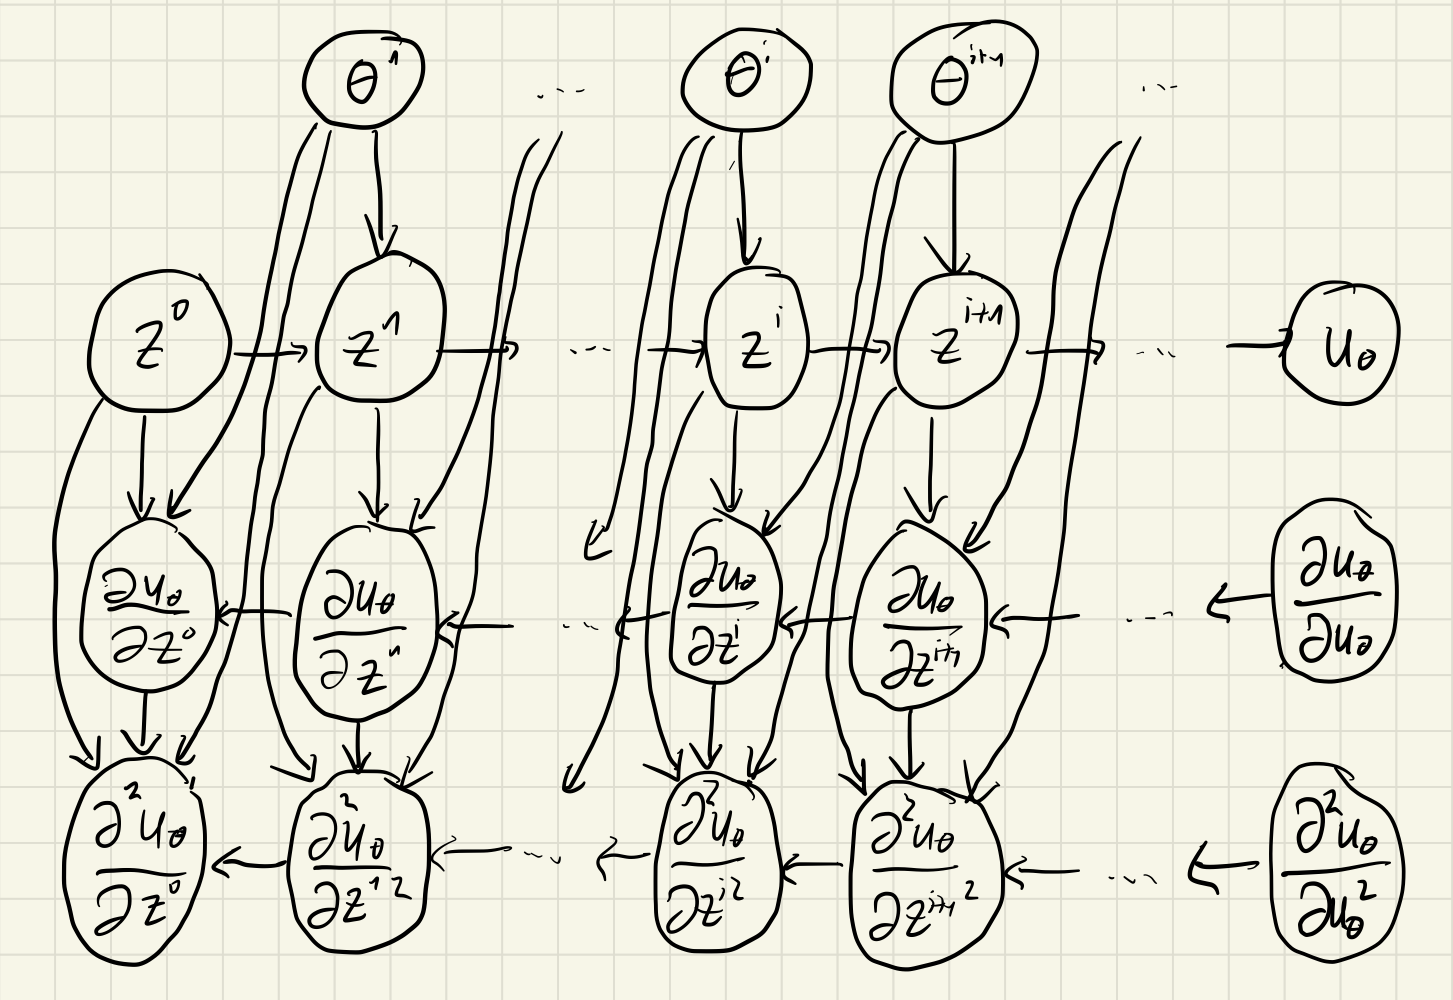
\includegraphics[width=0.6\linewidth]{figures/HBP_graph.png}
  \caption{Dependencies during gradient and Hessian backpropagation when computing the Hessian $\gradsquared{\vx}u_{\vtheta}$.}\label{fig:hbp-dependencies}
  \label{fig:hbp-dependencies}
\end{figure}

Following the procedure of \Cref{eq:hessian-backpropagation} yields the
per-layer parameter and feature Hessians $\gradsquared{\vz^{(i)}}u,
\gradsquared{\vtheta^{(i)}}u$. In \Cref{fig:hbp-dependencies} we depict the dependencies of
intermediate gradients and Hessians for computing $\gradsquared{\vx}u_{\vtheta}$:
\begin{itemize}
\item $\grad{\vz^{(i-1)}}u$ depends on $\grad{\vz^{(i)}}$ due to the recursion in \Cref{eq:gradient-backpropagation}, and on $\vz^{(i-1)}, \vtheta^{(i)}$ due to the Jacobian $\mJ_{\vz^{(i-1)}}\vz^{(i)}$ in the gradient backpropagation \Cref{eq:gradient-backpropagation}.

\item $\gradsquared{\vz^{(i-1)}}u$ depends on $\gradsquared{\vz^{(i)}}u$ and $\grad{\vz^{(i)}} u$ due to the recursion in \Cref{eq:hessian-backpropagation}, and on $\vz^{(i-1)}, \vtheta^{(i)}$ due to the Jacobian $\mJ_{\vz^{(i-1)}}\vz^{(i)}$ and Hessian $\gradsquared{\vz^{(i-1)}}[\vz^{(i)}]_k$ in the Hessian backpropagation \Cref{eq:gradient-backpropagation}.
\end{itemize}

\subsection{Laplacian}

The Laplacian $\Delta u_{\vtheta}$ follows by taking the trace of
$\gradsquared{\vx}u_{\vtheta}$ from above, and is hence recursively defined.

\begin{figure}[t]
  \centering
  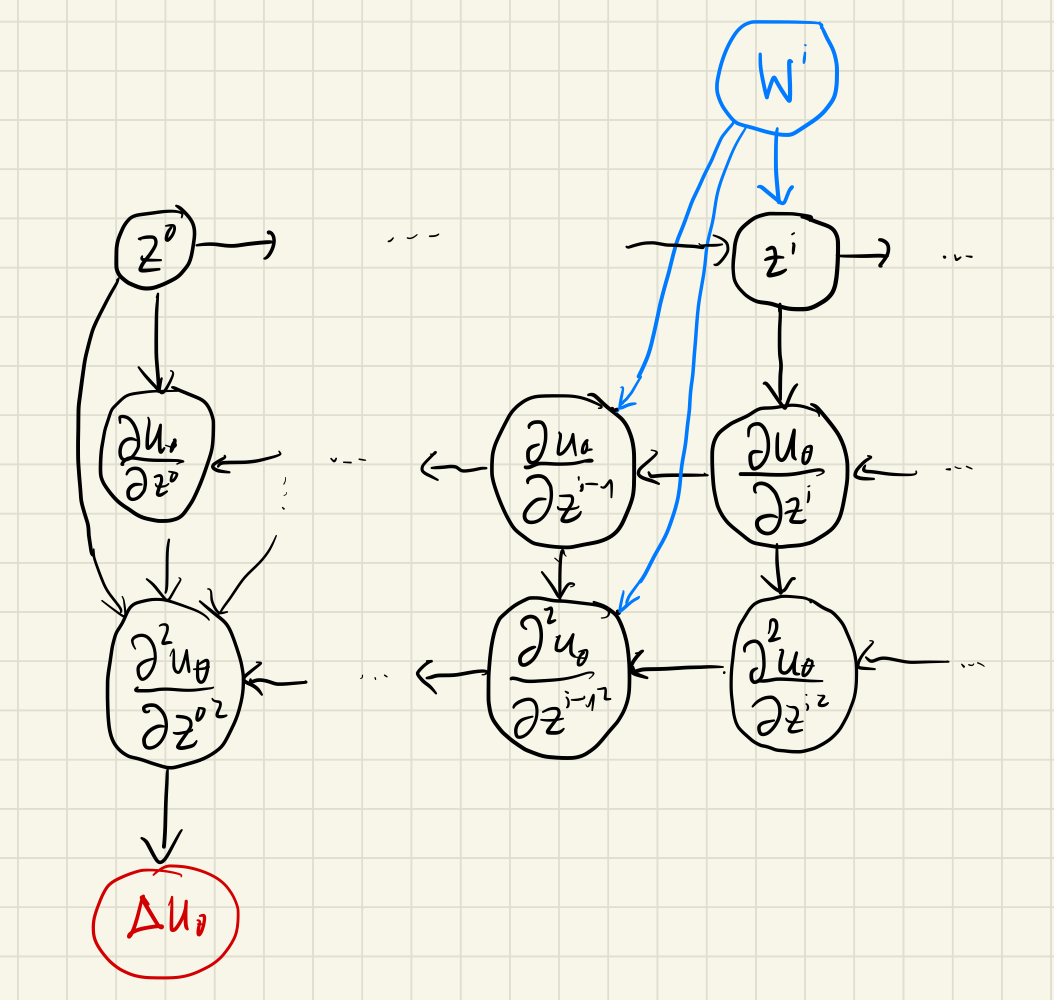
\includegraphics[width=0.6\linewidth]{figures/HBP_graph_weight.png}
  \caption{Direct children of the weight matrix of a single layer for the computation graph of the Laplacian.}\label{fig:laplacian-graph-weight}
\end{figure}

\paragraph{For a linear layer} To de-clutter the dependency graph of \Cref{fig:hbp-dependencies}, we will now consider the dependency of $\Delta u_{\vtheta}$ w.r.t.\,the weight of a single layer.
We assume this layer $i$ to be a linear layer with parameters $\mW^{(i)}$ such that $\vtheta^{(i)} = \flatten(\mW^{(i)})$,
\begin{align}
  \vz^{(i)} = \mW^{(i)} \vz^{(i-1)}\,.
\end{align}
For this layer, the second terms in \Cref{eq:hessian-backpropagation} disappears because the local Hessians are zero, that is $\gradsquared{\vz^{(i-1)}}[\vz^{(i)}]_k = \vzero$ and $\gradsquared{\mW^{(i)}}[\vz^{(i)}]_k = \vzero$.
Also, the Jacobians are $\jac_{\mW^{(i)}}\vz^{(i)} = {\vz^{(i-1)}}^{\top} \otimes \mI$ and $\jac_{\vz^{(i-1)}}\vz^{(i)} = \mW^{(i)}$ and hence only depends on one of the two layer inputs.
This simplifies the computation graph.
\Cref{fig:laplacian-graph-weight} shows the dependencies of $\mW^{(i)}$ on the
Laplacian, highlighting its three direct children,
\begin{align}
  \begin{split}
    \vz^{(i)}
    &=
      \mW^{(i)} \vz^{(i-1)}
    \\
    \grad{\vz^{(i-1)}}u
    &=
      {\mW^{(i)}}^{\top}
      \left(
      \grad{\vz^{(i)}}u
      \right)
    \\
    \gradsquared{\vz^{(i-1)}}u
    &=
      {\mW^{(i)}}^{\top}
      \left(
      \gradsquared{\vz^{(i)}}u
      \right)
      \mW^{(i)}
  \end{split}
\end{align}

\paragraph{Laplacian's derivative for a linear layer} We have now identified the direct children of $\mW^{(i)}$ in the Laplacian's compute graph.
This allows us to write down its derivative $\grad{\mW^{(i)}} \Delta u$, which---by the chain rule---is simply the accumulated backpropagated error from the direct children:
\begin{align}\label{eq:laplacian-gradient}
  \begin{split}
    \grad{\mW^{(i)}} \Delta u_{\vtheta}
    &=
      \sum_{\bullet \in \left\{ \vz^{(i)}, \grad{\vz^{(i-1)}}u, \gradsquared{\vz^{(i-1)}}u \right\}}
      \left(
      \jac_{\mW^{(i)}}\bullet
      \right)^{\top}
      \grad{\bullet}\Delta u
    \\
    &=
      \left(
      \jac_{\mW^{(i)}}\vz^{(i)}
      \right)^{\top}
      \grad{\vz^{(i)}}\Delta u
      +
      \left(
      \jac_{\mW^{(i)}}\grad{\vz^{(i)}}u
      \right)^{\top}
      \grad{\grad{\vz^{(i)}}u}\Delta u
      +
      \left(
      \jac_{\mW^{(i)}}\gradsquared{\vz^{(i)}}u
      \right)^{\top}
      \grad{\gradsquared{\vz^{(i)}}u}\Delta u\,.
  \end{split}
\end{align}

\paragraph{The Fisher} With the Laplacian's gradient \Cref{eq:laplacian-gradient}, we can write down the Fisher block for $\mW^{(i)}$
\begin{align}\label{eq:fisher}
  \begin{split}
    \mF^{(i)}
    &=
      \left(
      \grad{\mW^{(i)}} \Delta u_{\vtheta}
      \right)
      \left(
      \grad{\mW^{(i)}} \Delta u_{\vtheta}
      \right)^{\top}
    \\
    &=
      \sum_{\textcolor{blue}{\bullet} \in \left\{ \vz^{(i)}, \grad{\vz^{(i-1)}}u, \gradsquared{\vz^{(i-1)}}u \right\}}
      \sum_{\textcolor{red}{\bullet} \in \left\{ \vz^{(i)}, \grad{\vz^{(i-1)}}u, \gradsquared{\vz^{(i-1)}}u \right\}}
      \left(
      \left(
      \jac_{\mW^{(i)}}\textcolor{blue}{\bullet}
      \right)^{\top}
      \grad{\textcolor{blue}{\bullet}}\Delta u
      \right)
      \left(
      \left(
      \jac_{\mW^{(i)}}\textcolor{red}{\bullet}
      \right)^{\top}
      \grad{\textcolor{red}{\bullet}}\Delta u
      \right)^{\top}
    \\
    &=
      \sum_{\textcolor{blue}{\bullet} \in \left\{ \vz^{(i)}, \grad{\vz^{(i-1)}}u, \gradsquared{\vz^{(i-1)}}u \right\}}
      \sum_{\textcolor{red}{\bullet} \in \left\{ \vz^{(i)}, \grad{\vz^{(i-1)}}u, \gradsquared{\vz^{(i-1)}}u \right\}}
      \underbrace{
      \left(
      \jac_{\mW^{(i)}}\textcolor{blue}{\bullet}
      \right)^{\top}
      \left[
      \left(
      \grad{\textcolor{blue}{\bullet}}\Delta u
      \right)
      \left(
      \grad{\textcolor{red}{\bullet}}\Delta u
      \right)^{\top}
      \right]
      \left(
      \jac_{\mW^{(i)}}\textcolor{red}{\bullet}
      \right)}_{
      := \mF^{(i)}_{\textcolor{blue}{\bullet}, \textcolor{red}{\bullet}}
      }\,.
  \end{split}
\end{align}
The Fisher consists of nine different terms.
Eventually, we would like to approximate it with a single Kronecker product, like KFAC~\citep{martens2015optimizing}.
Note that one of the nine terms is the term from the original KFAC paper, namely
when $\textcolor{blue}{\bullet} = \textcolor{red}{\bullet} = \vz^{(i)}$
(remember that $\jac_{\mW^{(i)}} \vz^{(i)} = \vz^{(i-1)} \otimes \mI$):
\begin{align}\label{eq:original-kfac}
  \begin{split}
    \mF^{(i)}_{\textcolor{blue}{\vz^{(i)}}, \textcolor{red}{\vz^{(i)}}}
    &=
      \left(
      \textcolor{blue}{\vz^{(i-1)} \otimes \mI}
      \right)
      \left[
      \left(
      \textcolor{blue}{\grad{\vz^{(i-1)}}\Delta u}
      \right)
      \left(
      \textcolor{red}{\grad{\vz^{(i-1)}}\Delta u}
      \right)^{\top}
      \right]
      \left(
      \textcolor{red}{{\vz^{(i-1)}}^{\top} \otimes \mI}
      \right)
    \\
    &=
      \textcolor{blue}{\vz^{(i-1)}}
      \textcolor{red}{{\vz^{(i-1)}}^{\top}}
      \otimes
      \left(
      \textcolor{blue}{\grad{\vz^{(i-1)}}\Delta u}
      \right)
      \left(
      \textcolor{red}{\grad{\vz^{(i-1)}}\Delta u}
      \right)^{\top}
    \\
    &:= \mA_{\text{KFAC}}^{(i)} \otimes \mB_{\text{KFAC}}^{(i)}\,.
  \end{split}
\end{align}
\Cref{eq:original-kfac} illustrates that the Kronecker structure emerges from
the Jacobians. So we need to investigate these objects closer for the remaining
terms of \Cref{eq:fisher}.

\paragraph{Jacobians from the gradient and Hessian backward pass} We already know the Jacobian from the linear layer's forward pass,
\begin{subequations}\label{eq:fisher-jacobians}
  \begin{align}
    \jac_{\mW}\left( \mW \vx \right) = \vx^{\top} \otimes \mI\,.
  \end{align}
  The Jacobian from the gradient backpropagation is
  \begin{align}
    \jac_{\mW}\left( \mW^{\top} \vx \right) = \mI \otimes \vx^{\top}\,,
  \end{align}
  and the Jacobian from the Hessian backpropagation is
  \begin{align}
    \jac_{\mW}\left( \mW^{\top} \mX \mW \right) = \mI \otimes \mW^{\top}\mX + \mI \otimes \mW^{\top}\mX^{\top}\,.
  \end{align}
\end{subequations}
\toodoo{F.D.\,derived the Jacobians from \Cref{eq:fisher-jacobians} by hand.
  Might be worth to double-check for correctness.}
The Jacobians from \Cref{eq:fisher-jacobians} allow to express the Fisher in
terms of Kronecker-structured expressions consisting of 16 terms in total.

\toodoo{F.D.\,Write down the full expression for the Fisher.
  Propose ways to Kronecker-approximate each of the 16 terms, such that we end up with a single Kronecker product in the end.}

%%% Local Variables:
%%% mode: latex
%%% TeX-master: "../main"
%%% End:


\subsection{Kronecker Structure of the Gramian}\label{sec:kronecker-structure-gramian}

This subsection describes the Jacobians of the operations with the weight matrix in
a linear layer during the computation of the Laplacian and ends by providing an
equation for the Gramian block.

\toodoo{Propose ways to Kronecker-approximate the terms from identical children in to a single Kronecker product.}

\subsection{Kroneckerfactored Approximate Gramian (KFAG)}

This subsection describes the Kronecker approximation we propose for the per-layer Gramian.
It should also justify that the approximation is similar to that in other works.

\section{Generalization to other PDEs}

Essential to the formula above is that the discrete bilinear form (not explicitly stated above) can be written in the way
\begin{equation}\label{eq:gramian_asssumption}
  a^h(u,v)
  =
  \langle T(u), T(v) \rangle_{\mathbb R^N}.
\end{equation}
This implies
\begin{equation*}
  F(\theta) = D(T\circ P)^T \cdot D(T \circ P).
\end{equation*}
If you compute the entries of $F$ this yields
\begin{equation*}
  F(\theta)_{ij} = \langle T(\partial_{\theta_i}u_\theta), T(\partial_{\theta_j}u_\theta) \rangle_{\mathbb R^N}.
\end{equation*}
In the case of the Laplacian this $G$ will be one of the summands, so for example $F_\Omega$.
The map $T$ needs to be linear and is a combination of PDE operators and point evaluation, in the case of the Laplacian
\begin{equation*}
  T:C^2(\Omega) \to \mathbb R^{N_\Omega}, \quad T(u) = \frac{1}{\sqrt{N_{\Omega}}}(\Delta u(x_1), \dots, \Delta u(x_{N_{\Omega}})).
\end{equation*}
The map $P$ is the parametrization, i.e., $\theta\mapsto u_\theta$.
I think the form \eqref{eq:gramian_asssumption} is true for all of the PDEs we have in mind...but Johannes should double check that.

%%% Local Variables:
%%% mode: latex
%%% TeX-master: "../main"
%%% End:


\section{Experiments}

We want to show the following things:
\begin{itemize}
\item We can safely discard the Gramian's off-diagonal blocks without harming
  training performance. This reduces the Gramian's size, but still imposes
  strong constraints on scalability.

\item Our proposed Kronecker approximation works roughly as well as the
  full/block diagonal Gramian, while being much cheaper to compute, store, and
  invert.

\item Thanks to the Kronecker approximation of the Gramian, we can scale to larger neural networks where the other methods either do not work (storing the Gramian is prohibitibely expensive) or become quite slow (matrix-free linear system solve via Gramian-vector products).
\end{itemize}

Todos:
\begin{itemize}
\item concrete example ground truth: 2d Poisson on unit square with sine target
\end{itemize}

Ideas:
\begin{itemize}
\item try out different approximations
  \begin{itemize}
  \item Ground truth
  \item Block diagonal exact
  \item Diagonal
  \item Block diagonal with different approximations
  \end{itemize}
\end{itemize}

\section{Conclusion}

\paragraph{Limitations:}
\begin{itemize}
\item Only works for sequential networks
\item Hessian backpropagation requires memory quadratic in the intermediate features size and therefore becomes impractical for large intermediates like in CNNs.
\item Our implementation is likely manual and relatively hard to automate with the current graph inspection tools offered by ML frameworks.
\end{itemize}

\begin{ack} % automatically suppressed in anonymized submission
  The authors thank Runa Eschenhagen for insightful discussions on the relation to KFAC for weight sharing layers.
\end{ack}

\bibliography{references}
\bibliographystyle{apalike}

\appendix

\clearpage

% Use different numbering in appendix to make it clear that a
% section/table/algorithm is not in the main text
\renewcommand\thefigure{\thesection\arabic{figure}}
\renewcommand\thetable{\thesection\arabic{table}}
\renewcommand{\theequation}{\thesection\arabic{equation}}

% modified title header from main page, code extracted from NeurIPS template
\makeatletter
\vbox{%
  \hsize\textwidth
  \linewidth\hsize
  \vskip 0.1in
  \@toptitlebar
  \centering
  {\LARGE\bf \@title (Supplementary Material)\par}
  \@bottomtitlebar
  \vskip 0.3in \@minus 0.1in
}
\makeatother

% APPENDIX TOC
\startcontents[sections]
\printcontents[sections]{l}{1}{\setcounter{tocdepth}{2}}
\vspace{2em}

\section{The Computations for the Different KFACs}
\begin{equation*}
    \mG_\Omega(\mW^{(l)})
    =
    \frac1N\sum_{n=1}^N
    \left[\sum_{s=1}^S \left( \mZ^{(l-1)}_{n,s}\otimes \vg_{n,s}^{(l)} \right)
    \cdot
    \sum_{s=1}^S \left( \mZ
    ^{(l-1)}_{n,s}\otimes \vg_{n,s}^{(l)} \right)^\top\right]
\end{equation*}

%
%\paragraph{Kronecker approximation of the PDE Gramian}

\paragraph{The reduce approximation}
Approximating the sum of Kronecker products (running over $s$) by the Kronecker product of the sum, simplifying and again approximating for the outer sum (running over $n$) we obtain
\begin{align*}
    \hat{\mG}_\Omega^{\textup{red}}(\mW^{(l)})
    \coloneqq
    \frac{1}{N^2 S^2} \left[\sum_{n=1}^N \left( \sum_{s=1}^S \mZ^{(l-1)}_{n,s} \right) \left(\sum_{s=1}^S {\mZ^{(l-1)}_{n,s}}\right)^\top\right]
    \otimes
    \left[\sum_{n=1}^N\left(\sum_{s=1}^S \vg^{(l)}_{n,s} \right) \left( \sum_{s=1}^S {\vg^{(l)}_{n,s}} \right)^\top \right]
\end{align*}
This approximation agrees with the \emph{reduce} setting described by~\citet{eschenhagen2023kroneckerfactored}.

\paragraph{Individual steps} Can be moved to the appendix or deleted:

\begin{align*}
    &\; \sum_{n=1}^N
    \left[\sum_{s=1}^S \left( \mZ^{(l-1)}_{n,s}\otimes \vg_{n,s}^{(l)} \right)
    \cdot
    \sum_{s=1}^S \left( \mZ
    ^{(l-1)}_{n,s}\otimes \vg_{n,s}^{(l)} \right)^\top\right]
    \\ \approx & \;
    \sum_{n=1}^N
    \frac{1}{S^2}\left[\left(\left( \sum_{s=1}^S\mZ^{(l-1)}_{n,s}\right)\otimes \left(\sum_{s=1}^S\vg_{n,s}^{(l)}\right)\right)
    \cdot
    \left(\left( \sum_{s=1}^S\mZ^{(l-1)}_{n,s}\right)^\top\otimes \left(\sum_{s=1}^S\vg_{n,s}^{(l)}\right)^\top\right)\right]
    \\ = & \;
    \frac{1}{S^2}\sum_{n=1}^N
    \left[\left(\left( \sum_{s=1}^S\mZ^{(l-1)}_{n,s}\right)\left( \sum_{s=1}^S\mZ^{(l-1)}_{n,s}\right)^\top \right)\otimes \left(\left(\sum_{s=1}^S\vg_{n,s}^{(l)}\right)\left(\sum_{s=1}^S\vg_{n,s}^{(l)}\right)^\top\right)
     \right]
    \\ \approx & \;
    \frac{1}{N S^2}\left[\sum_{n=1}^N \left( \sum_{s=1}^S \mZ^{(l-1)}_{n,s} \right) \left(\sum_{s=1}^S {\mZ^{(l-1)}_{n,s}}\right)^\top\right]
    \otimes
    \left[\sum_{n=1}^N\left(\sum_{s=1}^S \vg^{(l)}_{n,s} \right) \left( \sum_{s=1}^S {\vg^{(l)}_{n,s}} \right)^\top \right]
\end{align*}


\paragraph{The expand approximation}
Alternatively, approximating the inner matrix product of sums in equation~\eqref{eq:laplace_gramian_block_exact} by the sum of matrix products, simplifying, and approximating the sum of Kroneckers by the Kronecker of the sum we obtain
\begin{align*}
    \hat{\mG}_\Omega^{\textup{exp}}(\mW^{(l)})
    \coloneqq \frac{1}{N^2 S}
    \left[\sum_{n=1}^N \sum_{s=1}^S \mZ^{(l-1)}_{n,s}{\mZ^{(l-1)}_{n,s}}^\top \right]
    \otimes
    \left[\sum_{n=1}^N\sum_{s=1}^S \vg^{(l)}_{n,s}{\vg^{(l)}_{n,s}}^\top   \right].
\end{align*}
which coincides with the \emph{expand} setting of \cite{eschenhagen2023kroneckerfactored}. 

\paragraph{Individual steps} 
An alternative to the approximation above, one can use the approximation $\sum_{n}A_n\sum_n B_n \approx N^{-1}\sum_{n}A_nB_n$ to get 
\begin{align*}
    & \sum_{n=1}^N
    \left[\sum_{s=1}^S \left( \mZ^{(l-1)}_{n,s}\otimes \vg_{n,s}^{(l)} \right)
    \cdot
    \sum_{s=1}^S \left( \mZ
    ^{(l-1)}_{n,s}\otimes \vg_{n,s}^{(l)} \right)^\top\right]
    \\ \approx & \;
    \frac{1}{S?}\sum_{n=1}^N
    \left[\sum_{s=1}^S \left( \mZ^{(l-1)}_{n,s}\otimes \vg_{n,s}^{(l)} \right)
    \cdot
    \left( \mZ
    ^{(l-1)}_{n,s}\otimes \vg_{n,s}^{(l)} \right)^\top\right]
    \\ = & \;
    \frac{1}{S}\sum_{n=1}^N
    \left[\sum_{s=1}^S \left( \mZ^{(l-1)}_{n,s}{\mZ
    ^{(l-1)}_{n,s}}^\top\otimes \vg_{n,s}^{(l)}{\vg_{n,s}^{(l)}}^\top \right)
    \right]
    \\ \approx & \;
    \frac{1}{NS}\left[\sum_{n=1}^N \sum_{s=1}^S \mZ^{(l-1)}_{n,s}{\mZ^{(l-1)}_{n,s}}^\top \right]
    \otimes
    \left[\sum_{n=1}^N\sum_{s=1}^S \vg^{(l)}_{n,s}{\vg^{(l)}_{n,s}}^\top \right].
\end{align*}


\section{Pseudo-Code: KFAC for the Poisson Equation}
\begin{algorithm}[!h]
  \centering
  \begin{small}
    \begin{algorithmic}
      \Require \\
      MLP $u_{\vtheta}$ with parameters $\vtheta_0 = (\vtheta_0^{(1)}, \dots, \vtheta_0^{(L)}) = (\flatten \mW_0^{(1)}, \dots, \flatten \mW_0^{(L)}) $, \\
      interior data $\{(\vx_n, y_n) \}_{n=1}^{N_{\Omega}}$, \\
      boundary data $\{(\vx^{\text{b}}_n, y^{\text{b}}_n) \}_{n=1}^{N_{\partial\Omega}}$ \\
      exponential moving average $\beta$, momentum $\mu$, Damping $\lambda$, number of steps $T$

      \\
      \State \textbf{0) Initialization}
      \For {$l=1, \dots, L$}
        \State $\mA_{\Omega}^{(l)}, \mB_{\Omega}^{(l)}, \mA_{\partial\Omega}^{(l)}, \mB_{\partial\Omega}^{(l)} \gets \vzero \text{ or } \mI$ \Comment Initialize Kronecker factors
      \EndFor
      \\
      \For {$t = 0, \dots, T-1$}
        \\
        \State \textbf{1) Compute the interior loss and update its approximate curvature}
        \State $(\mZ_n^{(0)}\dots, \mZ_n^{(L)}, \Delta u_n) \gets \Delta u_{\vtheta_t}(\vx_n)\quad n=1, \dots, N_{\Omega}$  \Comment Forward Laplacian wit intermediates

        \State Compute layer output gradients $\vg^{(l)}_{n,s} \coloneqq \nicefrac{\partial \Delta u_n}{\partial\mZ_{n,s}^{(l)}}$ with autodiff in one backward pass
        \State $(\vg_{n,s}^{(1)}, \dots, \vg_{n,s}^{(L)}) \gets \texttt{grad}(\Delta u_n, (\mZ_{n,s}^{(1)}, \dots, \mZ_{n,s}^{(L)}))\quad n=1, \dots, N_{\Omega}$, \quad $s = 1, \dots, S \coloneqq d+2$

        \ForAll{$l=1, \dots, L$} \Comment Update Kronecker factors of the interior loss
          \State $\hat{\mA}_{\Omega}^{(l)} \gets \beta \hat{\mA}_{\Omega}^{(l)} + (1-\beta) \frac1{N_{\Omega} S} \sum_{n=1}^{N_{\Omega}} \mZ_{n,s}^{(l-1)} \mZ_{n,s}^{(l-1)\top}$

          \State $\hat{\mB}_{\Omega}^{(l)} \gets \beta \hat{\mB}_{\Omega}^{(l)} + (1-\beta) \frac1{N_{\Omega}} \sum_{n=1}^{N_{\Omega}} \vg^{(l)}_{n,s} \vg^{(l)\top}_{n,s}$
        \EndFor

        \State $L_{\Omega}(\vtheta_t) \gets \frac{1}{2 N_{\Omega}}\sum_{n=1}^{N_{\Omega}} (\Delta u_n - y_n)^2$ \Comment Compute interior loss

        \\
        \State \textbf{2) Compute the boundary loss and update its approximate curvature}
        \State $(\vz_n^{(0)}\dots, \vz_n^{(L)}, u_n) \gets u_{\vtheta_t}(\vx_n^{\text{b}})\quad n=1, \dots, N_{\partial\Omega}$ \Comment Forward pass with intermediates
        \State Compute layer output gradients $\vg_n^{(l)} \coloneqq \nicefrac{\partial u_n}{\vz^{(l)}_n}$ with autodiff in one backward pass
        \State $(\vg_n^{(1)}\dots, \partial\vg_n^{(L)}) \gets \texttt{grad}(u_n, (\vz_n^{(0)}\dots, \vz_n^{(L)}))\quad n=1, \dots, N_{\partial\Omega}$

        \ForAll{$l=1, \dots, L$} \Comment Update Kronecker factors of the boundary loss
          \State $\hat{\mA}_{\partial\Omega}^{(l)} \gets \beta \hat{\mA}_{\partial\Omega}^{(l)} + (1-\beta) \frac1{N_{\partial\Omega}} \sum_{n=1}^{N_{\partial\Omega}} \vz_n^{(l-1)} \vz_n^{(l-1)\top}$

          \State $\hat{\mB}_{\partial\Omega}^{(l)} \gets \beta \hat{\mB}_{\partial\Omega}^{(l)} + (1-\beta) \frac1{N_{\partial\Omega}} \sum_{n=1}^{N_{\partial\Omega}} \vg_n^{(l)} \vg_n^{(l)\top}$
        \EndFor

        \State $L_{\partial\Omega}(\vtheta_t) \gets \frac{1}{2 N_{\partial\Omega}}\sum_{n=1}^{N_{\partial\Omega}} (u_n - y^{\text{b}}_n)^2$ \Comment Compute boundary loss

        \\
        \State \textbf{3) Update the preconditioner (use inverse of Kronecker sum trick)}
        \ForAll{$l=1, \dots, L$}
          \State $ \mC^{(l)} \gets \left[(\hat{\mA}_{\Omega}^{(l)} + \lambda \mI) \otimes (\hat{\mB}_{\Omega}^{(l)} + \lambda \mI) + (\hat{\mA}_{\partial\Omega}^{(l)} + \lambda \mI) \otimes (\hat{\mB}_{\partial\Omega}^{(l)} + \lambda \mI)  \right]^{-1}$
        \EndFor

        \\
        \State \textbf{4) Compute the gradient using autodiff, precondition the gradient}
        \State $(\vg^{(1)}, \dots, \vg^{(L)}) \gets \texttt{grad}( L_{\Omega}(\vtheta_t) + L_{\partial\Omega}(\vtheta_t), (\vtheta_t^{(1)}, \dots, \vtheta^{(L)}_t ))$ \Comment Gradient with autodiff

        \ForAll{$l=1, \dots, L$}
          \Comment Precondition gradient
          \State $\vDelta_t \gets - \mC^{(l)} \vg^{(l)}$ \Comment Proposed update direction
          \State $\hat{\vdelta}_t^{(l)} \gets \mu \vdelta_{t-1}^{(l)} + \vDelta_t^{(l)} \text{ if $t>0$ else } \vDelta_t^{(l)}$ \Comment Add momentum from previous update
        \EndFor

        \\
        \State \textbf{5) Given the direction $\hat{\vdelta}_t^{(1)}, \dots, \hat{\vdelta}_t^{(L)}$, choose learning rate $\alpha$ by line search \& update}
        \For {$l=1, \dots, L$} \Comment Parameter update
          \State $\vdelta_t^{(l)} \gets \alpha \hat{\vdelta}_t^{(l)}$
          \State $\vtheta^{(l)}_{t+1} \gets \vtheta^{(l)}_t + \alpha \vdelta_t^{(l)}$
        \EndFor
      \EndFor

      \\
      \State \Return Trained parameters $\vtheta_T$
    \end{algorithmic}
  \end{small}
    \caption{KFAC for the Poisson equation.}
\end{algorithm}
%%% Local Variables:
%%% mode: latex
%%% TeX-master: "../main"
%%% End:


%\section{Example: Laplacian for a Shallow Network}
%

\section{Example: Laplacian for a Shallow Network}

Here, we compute the Laplacian for a less general, yet simpler, example: A shallow neural network.

\begin{comment}
  For the one-dimensional shallow case we have
  \[ u_\theta(x) = \sum_{i=1}^m a_i\sigma(b_i x + c_i) + d. \]
  Then
  \[ u_\theta'(x) = \sum_{i=1}^m a_ib_i\sigma'(b_i x + c_i) \]
  and
  \[ u_\theta''(x) = \sum_{i=1}^m a_ib_i^2\sigma''(b_i x + c_i). \]
  The parameter derivative of the Laplacian (i.e., second-order derivative)
  \begin{align*}
    \partial_{a_i}u_\theta''(x) & = b_i^2\sigma''(b_i x + c_i) \\
    \partial_{b_i}u_\theta''(x) & = 2a_ib_i\sigma''(b_i x + c_i) + a_i b_i^2x\sigma^{(3)}(b_i x + c_i) \\
    \partial_{c_i}u_\theta''(x) & = a_i b_i^2\sigma^{(3)}(b_i x + c_i) \\
    \partial_{d}u_\theta''(x) & = 0.
  \end{align*}
  The parameter derivative of the Laplacian (i.e., second-order derivative)
  \begin{align*}
    \partial_{a_i}u_\theta''(x) & = b_i^2\sigma''(b_i x + c_i) \\
    \partial_{b_i}u_\theta''(x) & = 2a_ib_i\sigma''(b_i x + c_i) + a_i b_i^2x\sigma^{(3)}(b_i x + c_i) \\
    \partial_{c_i}u_\theta''(x) & = a_i b_i^2\sigma^{(3)}(b_i x + c_i) \\
    \partial_{d}u_\theta''(x) & = 0.
  \end{align*}
\end{comment}

First, we do the Hessian calculation as explicitly as possible. For this, we consider the easy case of a shallow network with one-dimensional output
\[ u_\theta(x) = \sum_{i=1}^m a_i\sigma(b_i^\top x + c_i) + d. \]
Then
\[ \nabla_x u_\theta(x) = \sum_{i=1}^m a_ib_i\sigma'(b_i x + c_i) \]
or
\[ \partial_{x_j} u_\theta(x) = \sum_{i=1}^m a_i(b_i)_j\sigma'(b_i x + c_i). \]
Consequently, we compute
\[ \partial_{x_k}\partial_{x_j} u_\theta(x) = \sum_{i=1}^m a_i(b_i)_j(b_i)_k\sigma'(b_i x + c_i) \]
which yields the Hessian
\[ \nabla^2_x u_\theta(x) = \sum_{i=1}^m a_i\sigma''(b_i x + c_i) \cdot b_ib_i^\top = \sum_{i=1}^m a_i\sigma''(b_i x + c_i) \cdot  b_i\otimes b_i \]
and the Laplacian is given by
\[ \Delta_x u_\theta(x) = \sum_{i=1}^m a_i\sigma''(b_i x + c_i) \operatorname{tr}(b_ib_i^\top) = \sum_{i=1}^m a_i\sigma''(b_i x + c_i)  \operatorname{tr}(b_i\otimes b_i). \]
The parameter derivatives of the Hessian are given
\begin{align*}
  \partial_{a_i}\nabla_x^2 u_\theta(x) & = \sigma''(b_i x + c_i) b_ib_i^\top \\
  \nabla_{b_i}\nabla_x^2 u_\theta(x) & = a_i\sigma''(b_i x + c_i) (b_i\otimes I+I\otimes b_i) + a_i \sigma^{(3)}(b_i x + c_i) \cdot  (I\otimes x^\top)(b_i\otimes b_i) \quad ?? \\
  % + a_i x\sigma^{(3)}(b_i x + c_i) \cdot b_ib_i^\top \\
     \partial_{c_i}\nabla_x^2 u_\theta(x) & = a_i b_i^2\sigma^{(3)}(b_i x + c_i) \\
     \partial_{d}\nabla_x^2 u_\theta(x) & = 0.
\end{align*}
The parameter derivatives of the Laplacian are given
\begin{align*}
     \partial_{a_i}\Delta_x u_\theta(x) & = \sigma''(b_i x + c_i) \operatorname{tr}(b_ib_i^\top) \\
     \nabla_{b_i}\Delta_x u_\theta(x) & = 2a_i\sigma''(b_i x + c_i) + a_i \sigma^{(3)}(b_i x + c_i) \operatorname{tr}(b_ib_i^\top) \cdot x \\
     \partial_{c_i}\Delta_x u_\theta(x) & = a_i \sigma^{(3)}(b_i x + c_i)\operatorname{tr}(b_ib_i^\top) \\
     \partial_{d}\Delta_x u_\theta(x) & = 0.
\end{align*}


\paragraph{Writing as linear algebra}

Consider a shallow network
\[ u_\theta(x) = W_2\sigma(W_1 x), \]
where $x\in\mathbb R^d$, $W_1\in\mathbb R^{m\times d}, W_2\in\mathbb R^{1\times m}$.

\paragraph{Task: }
Understand the structure, in particular the computational graph of $f_\theta = \Delta u_\theta$.

\paragraph{One dimensional case: }
Assume first that $d=1$.
Then
\[ D_x u_\theta(x) = W_2 \operatorname{diag}(\sigma'(W_1 x)) W_1 \]
and
\[ D^2_x u_\theta(x) = W_2%(W_1^\top\otimes W_2)
  \operatorname{diag}(\operatorname{diag}(\sigma''(W_1 x)) W_1)W_1. % = W_2 \operatorname{diag}\sigma''(W_1 x) W_1^2 = W_2\odot W_1^2 \sigma''(W_1x),
\]
In another form
\[D^2 u_\theta(x) = W_2 \operatorname{diag}(\operatorname{diag}\sigma''(W_1 x) W_1) W_1 = W_2 \operatorname{diag}\sigma''(W_1 x) W_1^2 = W_2\odot W_1^2 \sigma''(W_1x),
\]
where $(W_2\odot W_1^2)_k = (W_2)_k \cdot (W_1)_k^2$.
% where $(W_2\odot W_1^2)_k = (W_2)_k \cdot (W_1)_k^2$.
% The Laplacian is then given as
% \[ f_\theta(x) = \Delta u_\theta(x) = \operatorname{tr}(D_x^2u_\theta(x)) =\operatorname{tr}(W_2 \operatorname{diag}(\operatorname{diag}(\sigma''(W_1 x)) W_1) W_1).  \]
% Differentiation with respect to $W_2$ yields
% \[ \frac{\partial f_\theta(x)}{\partial W_2} = \frac{\partial \Delta u_\theta(x)}{ \partial W_2} =  \]

One can also rewrite the diagonalization operator via a Hadamard product as $\operatorname{diag}(x) = (x\mathds{1}^\top)\odot I$, where $\mathds{1}$ denotes the all one vector, $I$ the identity and $\odot$ the Hadamard (i.e., entrywise) product of two matrices.
Not sure whether this helps though...

\paragraph{Multi-dimensional case}

%%% Local Variables:
%%% mode: latex
%%% TeX-master: "../main"
%%% End:


\section{Inverting the Sum of Two Kronecker Matrices}\label{sec:inverse_kronecker_sum}
PINNs use two losses: a boundary and an interior loss.
When designing a Kronecker-factored curvature approximation, we have two choices:
\begin{enumerate}
\item We can approximate each loss individually with a Kronecker product, i.e.
  \begin{align*}
    \mK \coloneqq \mA_1 \otimes \mA_2 + \mB_1 \otimes \mB_2
  \end{align*}
  where $\mA_{1,2}, \mB_{1,2}$ are invertible and positive definite.

\item We can further approximate the above through a single Kronecker product, e.g.\,by summing,
  \begin{align*}
    \mK' \coloneqq (\mA_1 + \mB_1) \otimes (\mA_2 + \mB_2) \approx \mK\,.
  \end{align*}
\end{enumerate}
Eventually, we want to use their inverses.
For $\mK'$, this is straightforward to do.
For $\mK$, we need to invert the sum of two Kronecker products, which is more challenging.
We can proceed as follows to invert $\mK$:
\begin{enumerate}
\item Simultaneously diagonalize $(\mA_i, \mB_i)$ by solving the generalized eigenvalue problem
  \begin{align*}
    \mA_i \mV_i = \mB \mV_i \mLambda_i
  \end{align*}
  where $\mV_i$'s columns are the (generalized) eigenvectors and $\mLambda_i$ is a diagonal matrix containing the (generalized) eigenvalues.

\item Consider the expression
  \begin{align*}
    &\left(
      \mA_1 \otimes \mA_2
      +
      \mB_1 \otimes \mB_2
      \right)
      \left(
      \mV_1 \otimes \mV_2
      \right)
    \\
    &=
      \mB_1 \mV_1 \mLambda_1 \otimes \mB_2 \mV_2 \mLambda_2
      +
      \left( \mB_1 \otimes \mB_2 \right)
      \left( \mV_1 \otimes \mV_2 \right)
    \\
    &=
      \left( \mB_1 \otimes \mB_2 \right)
      \left( \mV_1 \otimes \mV_2 \right)
      \left(
      \mLambda_1 \otimes \mLambda_2 + \mI \otimes \mI
      \right)\,.
  \end{align*}
  Rearrange into
  \begin{align*}
    \left(
    \mA_1 \otimes \mA_2
    +
    \mB_1 \otimes \mB_2
    \right)
    =
    \left( \mB_1 \otimes \mB_2 \right)
    \left( \mV_1 \otimes \mV_2 \right)
    \left(
    \mLambda_1 \otimes \mLambda_2 + \mI \otimes \mI
    \right)
    \left( \mV_1^{-1} \otimes \mV_2^{-1} \right)
    \,.
  \end{align*}

  \item Take the inverse to obtain
    \begin{align*}
      \mK^{-1}
      =
      \left( \mV_1 \otimes \mV_2 \right)
      \left(
      \mLambda_1 \otimes \mLambda_2 + \mI \otimes \mI
      \right)^{-1}
      \left( \mV_1^{-1}\mB_1^{-1} \otimes \mV_2^{-1}\mB_2^{-1} \right)
      \,.
    \end{align*}
    Notice that $\mLambda_1 \otimes \mLambda_2 + \mI \otimes \mI$ is diagonal, and therefore easy to invert.
\end{enumerate}

%%% Local Variables:
%%% mode: latex
%%% TeX-master: "../main"
%%% End:


%\section{Heat Equation}\label{sec:heat_equation}
%Consider the $D$-dimensional\todo{Low priority: lower case $d$ or upper case $D$? The number of trainable weights is already $D$.} homogeneous heat equation
\begin{align*}
  \partial_{t} u(t, \vx)
  -
  \kappa \Delta_{\vx} u(t, \vx)
  =
  0
\end{align*}
where $\vx \in \Omega \subseteq \sR^D$, $t \in \mathrm{T} \subseteq \sR$ is a time interval, and $\kappa >0$ denotes the heat conductivity. In this case, our neural network processes a $D+1$-dimensional vector $\tilde{\vx} =
\begin{pmatrix} t \\ \vx \end{pmatrix}$ and we can re-write the heat equation as
\begin{align*}
  \partial_{[\tilde{\vx}]_1} u(\tilde{\vx})
  -
  \kappa \sum_{d=2}^{D+1} \Delta_{[\tilde{\vx}]_d} u(\tilde{\vx})
  =
  0\,.
\end{align*}
In the following, we consider the unit time interval $\mathrm{T} = [0;1]$, the unit square $\Omega = [0;1]^D$ and set $\kappa = \nicefrac{1}{4}$. There are two types of constraints we need to enforce on the heat equation in order to obtain unique solutions: initial conditions and boundary conditions. As our framework for the KFAC approximation assumes only two terms in the loss function, we combine the contributions from the boundary and initial values into one term. To make this more precise consider the following example solution of the heat equation, which will be used later on as well.
As initial conditions, we use $u_0(x) = u(0, \vx) = \prod_{d=1}^D \sin(\pi [\vx_d])$ for $\vx \in \Omega$.
For boundary conditions, we use $g(t, \vx) = 0$ for $t, \vx \in \mathrm{T} \times \partial\Omega$.
The manufactured solution thus is
\begin{align*}
  u^{\star}(t, \vx)
  =
  \exp \left(-\frac{\pi^2 D t}{4} \right)
  \prod_{d=1}^D \sin(\pi [\vx_d])\,.
\end{align*}
The PINN loss for this problem consists of three terms
\begin{align*}
  \gL(\vtheta)
  &=
    \frac{1}{N_{\Omega}}
    \sum_{n=1}^{N_{\Omega}}
    \left\lVert
    \partial_t u_{\vtheta}(\tilde{\vx}_n^{\Omega})
    -
    \frac{1}{4} \Delta_{\vx} u_{\vtheta}(\tilde{\vx}_n^{\Omega})
    \right\rVert^2_2
  \\
  &+
    \frac{1}{N_{\partial\Omega}}
    \sum_{n=1}^{N_{\partial\Omega}}
    \left\lVert
    u_{\vtheta}(\tilde{\vx}_n^{\partial\Omega})
    -
    g(\tilde{\vx}_n^{\partial\Omega})
    \right\rVert^2_2
  \\
  &+
    \frac{1}{N_0}
    \sum_{n=1}^{N_0}
    \left\lVert
    u_{\vtheta}(0, \vx_n^0)
    -
    u_0( \vx_n^0)
    \right\rVert^2_2
\end{align*}
with $\tilde{\vx}_n^{\Omega} \sim \mathrm{T} \times \Omega$, and $\tilde{\vx}_n^{\partial\Omega} \sim \mathrm{T} \times \partial\Omega$, and $\vx_n^0 \sim \{0\} \times \Omega$.
To fit this loss into our framework which assumes two loss terms, each of whose curvature is approximated with a Kronecker factor, we combine the initial value and boundary value conditions into a single term.
Assuming $N_{\partial \Omega} = N_0 = \nicefrac{N_{\text{cond}}}{2}$ without loss of generality, we write
\begin{align*}
  \gL(\vtheta)
  &=
    \underbrace{
    \frac{1}{N_{\Omega}}
    \sum_{n=1}^{N_{\Omega}}
    \left\lVert
    \partial_t u_{\vtheta}(\tilde{\vx}_n^{\Omega})
    -
    \frac{1}{4} \Delta_{\vx} u_{\vtheta}(\tilde{\vx}_n^{\Omega})
    - y_n^{\Omega}
    \right\rVert^2_2
    }_{\gL_{\Omega}(\vtheta)}
  +
    \underbrace{
    \frac{1}{N_{\text{cond}}}
    \sum_{n=1}^{N_{\text{cond}}}
    \left\lVert
    u_{\vtheta}(\tilde{\vx}_n^{\text{cond}})
    -
    y_n^{\text{cond}}
    \right\rVert^2_2
    }_{\gL_{\text{cond}}(\vtheta)}
\end{align*}
with domain inputs $\tilde{\vx}_n^{\Omega} \sim \mathrm{T} \times \Omega$ and targets $y_n^{\Omega} = 0$, boundary and initial condition targets $y_n^{\text{cond}} = u(\tilde{\vx}_n^{\text{cond}})$ with initial inputs $\tilde{\vx}_n^{\text{cond}} \sim \{0\} \times \Omega$ for $n = 1, \dots, \nicefrac{N_{\text{cond}}}{2}$ and boundary inputs $\tilde{\vx}_n^{\partial\Omega} \sim \mathrm{T} \times \partial\Omega$ for $n = \nicefrac{N_{\text{cond}}}{2}+1, \dots, N_{\text{cond}}$.
The boundary and initial condition loss are of exactly same structure as the loss we discussed for the Poisson equation.

%%% Local Variables:
%%% mode: latex
%%% TeX-master: "../main"
%%% End:


%\section{Taylor-Mode Automatic Differentiation \& Forward Laplacian}
%PINN losses involve differential operators of the neural network, for instance the Laplacian.
Recently, \citet{li2023forward} proposed a new computational framework called \emph{forward Laplacian} to evaluate the Laplacian and the neural network's prediction in one forward traversal.
To establish a Kronecker-factorized approximation of the Gramian, which consists of the Laplacian's gradient, we need to know how a weight matrix enters its computation.
Here, we describe how the weight matrix of a linear layer inside a feed-forward net enters the Laplacian's computation when using the forward Laplacian framework.
We start by connecting the forward Laplacian framework to Taylor-mode automatic differentiation \citep{griewank2008evaluating,bettencourt2019taylor}, both to make the presentation self-contained and to explicitly point out this connection which we believe has not been done previously.

\subsection{Taylor-Mode Automatic Differentiation}\label{sec:taylor-mode-tutorial}
The idea of Taylor-mode is to forward-propagate Taylor coefficients, i.e.\,directional derivatives, through the computation graph. We provide a brief summary based on its description in \cite{bettencourt2019taylor}.

\paragraph{Taylor series and directional derivatives} Consider a function $f: \sR^d \to \sR$ and its $K$-th order Taylor expansion at a point $\vx \in \sR^d$ along a direction $\alpha \vv \in \sR^d$ with $\alpha \in \sR$,
\begin{align*}
  \hat{f}(\alpha) =
  f(\vx + \alpha \vv)
  &=
    f(\vx)
    +
    \alpha
    \left(
    \frac{\partial f(\vx)}{\partial \vx}
    \right)^{\top} \vv
    +
    \frac{\alpha^2}{2!}
    \vv^\top
    \left(
    \frac{\partial^2 f(\vx)}{\partial \vx^2}
    \right) \vv
  \\
  &\phantom{=}+
    \frac{\alpha^3}{3!}
    \sum_{i_1, i_2 i_3}
    \left(
    \frac{\partial^3 f(\vx)}{\partial\vx^3}
    \right)_{i_1, i_2, i_3} \evv_{i_1} \evv_{i_2} \evv_{i_3}
  \\
  &\phantom{=}+
    \ldots
  \\
  &\phantom{=}+
    \frac{\alpha^K}{K!}
    \sum_{i_1, \dots, i_K}
    \left(
    \frac{\partial^K f(\vx)}{\partial\vx^K}
    \right)_{i_1, \dots, i_K} \evv_{i_1} \cdots \evv_{i_K}\,.
\end{align*}
We can unify this expression by introducing the $K$-th order directional derivative of $f$ at $\vx$ along $\vv$,
\begin{align*}
  \partial^K f(\vx)
  \underbrace{\left[ \vv, \ldots, \vv \right]}_{K\,\text{times}}
  \coloneqq
  \sum_{i_1, \dots, i_K}
  \left(
  \frac{\partial^K f(\vx)}{\partial\vx^K}
  \right)_{i_1, \dots, i_K} \evv_{i_1} \dots \evv_{i_K}\,.
\end{align*}
This simplifies the uni-directional Taylor expansion to
\begin{align*}
  \hat{f}(\alpha) = f(\vx + \alpha\vv)
  &=
    f(\vx)
    +
    \alpha
    \partial f(\vx)[\vv]
    +
    \frac{\alpha^2}{2!}
    \partial^2 f(\vx)[\vv, \vv]
    +
    \frac{\alpha^3}{3!}
    \partial^3 f(\vx)[\vv, \vv, \vv]
  \\
  &\phantom{=}+
    \ldots
    +
    \frac{\alpha^K}{K!}
    \partial^K f(\vx)[\vv, \ldots, \vv]
  \\
  &\eqqcolon
    \sum_{k=1}^K
    \frac{\alpha^k}{k!}
    \partial^k f(\vx)\left[\otimes^k \vv  \right]
    \eqqcolon
    \sum_{k=1}^K
    w^f_k \alpha^k
\end{align*}
where we have used the notation $\otimes^k \vv$ to indicate $k$ copies of $\vv$, and introduced the $k$-th order Taylor coefficient $w^f_k \in \sR$ of $f$.
This generalizes to vector-valued functions:
If $f$'s output was vector-valued, say $f(\vx) \in \sR^c$, we would have Taylor-expanded each component individually and grouped coefficients of same order into vectors $\vw_k^f \in \sR^c$ such that $[\vw_k^f]_i$ is the $k$-th order Taylor coefficient of the $i$th component of $f$.

\paragraph{A note on generality:} In this introduction to Taylor-mode, we limit the discussion to the computation of higher-order derivatives along a single direction $\vv$, i.e.\,$\partial^Kf(\vx)[\vv, \dots, \vv]$.
This is limited though, e.g.\,if we set $K=2$ then we can compute $\partial^2 f(\vx)[\vv, \vv] = \vv^{\top} (\nicefrac{\partial^2 f(\vx)}{\partial\vx^2}) \vv$.
We can set $\vv = \ve_i$ to the $i$-th standard basis vector to compute the $i$-th diagonal element of the Hessian.
But we cannot evaluate off-diagonal elements, as this would require multi-directional derivatives, like $\partial^2 f(\vx) [\ve_i, \ve_{j\neq i}]$.
A more general description of Taylor-mode for multi-directional Taylor series along $M$ directions, $\hat{f}(\alpha_1, \dots, \alpha_M) = f(\vx + \alpha_1 \vv_1 + \dots + \alpha_M \vv_M)$, which require more general directional derivatives $\partial^K f(\vx) [\vv_1, \dots, \vv_K]$ (each vector can be different) are discussed in \cite{johnson2021taylor-made}.
We will use this formulation later to generalize the forward Laplacian scheme to more general weighted sums of second-order derivatives in \Cref{sec:generalized-forward-laplacian}.

\paragraph{Composition rule}
Next, we consider the case where $f = g \circ h$ is a composition of two functions. Starting from the Taylor coefficients $\vw_0^h, \dots \vw_K^h$ of $\hat{h}(\alpha) = h(\vx + \alpha \vv)$, the Taylor coefficients $\vw_0^f, \dots, \vw_K^f$ of $\hat{f}(\alpha) = f(\vx + \alpha\vv)$ follow from Fa\`a di Bruno's formula~\cite{griewank2008evaluating,bettencourt2019taylor}:
\begin{align}\label{eq:taylor-mode-forward}
  \vw_{k}^f
  =
  \sum_{\sigma \in \mathrm{part}(k)}
  \frac{1}{n_1! \dots n_K!}
  \partial^{|\sigma|}g(\vw_0^h)
  \left[
  \otimes_{s \in \sigma}
  \vw_s^h
  \right]
\end{align}
In the above, $\mathrm{part}(k)$ is the set of all integer partitionings of $k$; a set of sets. $|\sigma|$ denotes the length of a set $\sigma \in \mathrm{part}(k)$, $n_i$ is the count of integer $i$ in $\sigma$, and $\vw_0^h = h(\vx)$.

\textbf{Second-order Taylor-mode} Our goal is the computation of second-order derivatives of $f$ w.r.t.\,$\vx$.
So let's work out \Cref{eq:taylor-mode-forward} up to order $K=2$.
The zeroth and first order are simply the forward pass and the forward-mode gradient chain rule.
For the second-order term, we need the integer partitioning of 2, given by $\mathrm{part}(2) = \left\{ \{1, 1\}, \{2\} \right\}$.
This results in
\begin{subequations}\label{eq:taylor-mode-second-order}
  \begin{align}
    \vw_0^f
    &=
      g(\vw_0^h)\,,
    \\
    \vw_1^f
    &=
      \partial g(\vw_0^h)[\vw_1^h]\,,
    \\
    \vw_2^f
    &=
      \frac{1}{2}
      \partial^2 g(\vw_0^h)[\vw_1^h, \vw_1^h]
      +
      \partial g(\vw_0^h)[\vw_2^h]\,.
  \end{align}
\end{subequations}
We can also express $\vw_1^f, \vw_2^f$ in terms of Jacobian- and Hessian-vector products of $g$,
\begin{subequations}\label{eq:taylor-mode-second-order-jac-hess}
  \begin{align}
    \label{eq:taylor-mode-second-order-jac}
    \vw_1^f
    &=
      \left(
      \jac_{\vw_0^h} g(\vw_0^h)
      \right) \vw_1^h\,,
    \\
    \vw_2^f
    &=
      \frac{1}{2}
      \begin{pmatrix}
        {\vw_1^h}^{\top}
        \frac{
        \partial^2 \left[ g(\vw_0^h) \right]_1
        }{
        \partial{\vw_0^h}^2
        }
        \vw_1^h
        \\
        \vdots
        \\
        {\vw_1^h}^{\top}
        \frac{
        \partial^2 \left[ g(\vw_0^h) \right]_D
        }{
        \partial{\vw_0^h}^2
        }
        \vw_1^h
      \end{pmatrix}
      +
      \left(
      \jac_{\vw_0^h} g(\vw_0^h)
      \right) \vw_2^h\,.
  \end{align}
\end{subequations}
Note that first-order Taylor-mode (\Cref{eq:taylor-mode-second-order-jac}) corresponds to the standard forward-mode autodiff which pushes forward error signals through Jacobian-vector products.

\subsection{Forward Laplacian}
Our goal is to compute the Laplacian of $f: \sR^d \to \sR^c$ (in practise, $c=1$),
\begin{align}
  \Delta_{\vx} f(\vx)
  =
  \sum_{i=1}^d
  \begin{pmatrix}
    \partial^2[f(\vx)]_1[\ve_i, \ve_i]
    \\
    \vdots
    \\
    \partial^2[f(\vx)]_c[\ve_i, \ve_i]
  \end{pmatrix}
  \coloneq
  2 \sum_{i=1}^d \vw_{2,i}^f \in \sR^c\,,
\end{align}
where $\ve_i$ is the $i$-th standard basis vector, $[f(\vx)]_j$ is the $j$-th component of $f(\vx)$, and we have introduced the second-order Taylor coefficients $\vw_{2,i}^f$ of $f$ along $\ve_i$.
The Laplacian requires computing, then summing, the second-order Taylor coefficients of $d$ Taylor approximations $\{f(\vx + \ve_i)\}_{i=1,\dots, d}$.

\paragraph{Naive approach} We can use Taylor-mode differentiation to compute all these components in one forward traversal. Adding the extra loop over the Taylor expansions we want to compute in parallel, we obtain the following scheme from \Cref{eq:taylor-mode-second-order},
\begin{subequations}\label{eq:taylor-mode-naive-laplacian}
  \begin{align}
    \vw_0^f
    &=
      g(\vw_0^h)\,,
    \\
    \left\{
    \vw_{1,i}^f
    \right\}_{i=1, \dots, d}
    &=
      \left\{
      \partial g(\vw_0^h)[\vw_{1,i}^h]
      \right\}_{i=1, \dots, d}\,,
    \\ \label{eq:naive-laplacian-second-order-term}
    \left\{
    \vw_{2,i}^f
    \right\}_{i=1, \dots, d}
    &=
      \left\{
      \frac{1}{2}
      \partial^2 g(\vw_0^h)[\vw_{1,i}^h, \vw_{1,i}^h]
      +
      \partial g(\vw_0^h)[\vw_{2,i}^h]
      \right\}_{i=1, \dots, d}\,.
  \end{align}
\end{subequations}

\paragraph{Forward Laplacian framework}
Computing the Laplacian via \Cref{eq:taylor-mode-naive-laplacian} first computes, then sums, the diagonal second-order derivatives $\{ \vw_{2,i}^f \}_{i=1,\dots, d}$.
Note that we can pull the sum inside the forward propagation scheme, specifically \Cref{eq:naive-laplacian-second-order-term}, and push-forward the summed second-order coefficients. This simplifies \Cref{eq:taylor-mode-naive-laplacian} to
\begin{subequations}\label{eq:forward-laplacian}
  \begin{align}
    \vw_0^f
    &=
      g(\vw_0^h)\,,
    \\
    \left\{
    \vw_{1,i}^f
    \right\}_{i=1, \dots, d}
    &=
      \left\{
      \partial g(\vw_0^h)[\vw_{1,i}^h]
      \right\}_{i=1, \dots, d}\,,
    \\
    \underbrace{
    \sum_{i=1}^d
    \vw_{2,i}^f
    }_{\nicefrac{1}{2}\Delta_{\vx} f(\vx)}
    &=
      \left(
      \frac{1}{2}
      \sum_{i=1}^d
      \partial^2 g(\vw_0^h)[\vw_{1,i}^h, \vw_{1,i}^h]
      \right)
      +
      \partial g(\vw_0^h)
      \underbrace{
      \left[
      \sum_{i=1}^d \vw_{2,i}^h
      \right]
      }_{\nicefrac{1}{2}\Delta_{\vx} g(\vx)}\,.
  \end{align}
\end{subequations}
\Cref{eq:forward-laplacian} is the forward Laplacian framework from \citet{li2023forward} for computing the Laplacian of a neural network.
Here, we have derived it from Taylor-mode automatic differentiation.
Note that \Cref{eq:forward-laplacian} requires less computations and memory than \Cref{eq:taylor-mode-naive-laplacian} because we can pull the summation from the Laplacian into the forward propagation scheme.

\subsubsection{Forward Laplacian for Elementwise Activation Layers}
We now describe \Cref{eq:forward-laplacian} for the case where $g: \sR^c \to \sR^c$ acts element-wise via $\sigma: \sR \to \sR$.
We will write $\sigma(\bullet), \sigma'(\bullet), \sigma''(\bullet)$ to indicate element-wise application of $\sigma$, its first derivative $\sigma'$, and second derivative $\sigma''$ to all elements of $\bullet$.
Further, let $\odot$ denote element-wise multiplication, and $(\bullet)^{\odot 2}$ element-wise squaring.
With that, we can write the Jacobian as $\jac_{h(\vx)}g(\vx) = \diag(\sigma(h(\vx)))$ where $\diag(\bullet)$ embeds a vector $\bullet$ into the diagonal of a matrix.
The Hessian of component $i$ is $\nicefrac{\partial^2 [g(h(\vx))]_i}{\partial h(\vx)^2} = [\sigma''(h(\vx))]_i \ve_i \ve_i^{\top}$.
Inserting \Cref{eq:taylor-mode-second-order-jac-hess} into \Cref{eq:forward-laplacian} and using the Jacobian and Hessian expressions of the element-wise activation function yields the following forward Laplacian forward propagation:
\begin{subequations}\label{eq:forward-laplacian-activation-layers}
  \begin{align}
    \vw_0^f
    &=
      \sigma(\vw_0^h)\,,
    \\
    \left\{ \vw_{1,i}^f \right\}
    &=
      \left\{ \sigma'(\vw_0^h) \odot \vw_{1,i}^h \right\}_{i=1, \dots, d}\,,
    \\
    \sum_{i=1}^d \vw_{2,i}^f
    &=
      \frac{1}{2}
      \sigma''(\vw_0^h) \odot
      \left(
      \sum_{i=1}^d
      \left(\vw_{1,i}^h\right)^{\odot 2}
      \right)
      +
      \sigma'(\vw_0^h)
      \odot
      \left(
      \sum_{i=1}^d \vw_{2,i}^h
      \right)\,.
  \end{align}
\end{subequations}

\subsubsection{Forward Laplacian for Linear Layers}
Now, let $g: \sR^{D_{\text{in}}} \to \sR^{D_{\text{out}}}$ be a linear layer with weight matrix $\mW \in \sR^{D_{\text{out}} \times D_{\text{in}}}$ and bias vector $\vb \in \sR^{D_{\text{out}}}$.
Its Jacobian is $\jac_{h(\vx)}( \mW h(\vx) + \vb) = \mW$ and the second-order derivative is zero.
Hence, \Cref{eq:forward-laplacian} for linear layers becomes
\begin{subequations}\label{eq:forward-laplacian-linear-layer}
  \begin{align}
    \vw_0^f
    &=
      \mW \vw_0^h + \vb\,,
    \\
    \left\{ \vw_{1,i}^f \right\}_{i=1, \dots, d}
    &=
      \left\{ \mW \vw_{1,i}^h \right\}_{i=1, \dots, d}\,,
    \\
    \sum_{i=1}^d \vw_{2,i}^f
    &=
      \mW
      \left( \sum_{i=1}^d \vw_{2,i}^h\right)\,.
  \end{align}
\end{subequations}
We can summarize \Cref{eq:forward-laplacian-linear-layer} in a single equation by grouping all quantities that are multiplied by $\mW$ into a single matrix, and appending a single row of ones or zeros to account for the bias:
\begin{align}
  \nonumber
  \underbrace{
  \begin{pmatrix}
    \vw_0^f
    &
      \vw_{1,1}^f
    &
      \dots
    &
      \vw_{1,d}^f
    &
      \sum_{i=1}^D \vw_{2,i}^f
  \end{pmatrix}
  }_{\coloneq \mT^f \in \sR^{D_{\text{out}} \times (d+2)}}
  &=
    \begin{pmatrix}
      \mW & \vb
    \end{pmatrix}
    \underbrace{
    \begin{pmatrix}
      \vw_0^h
      &
        \vw_{1,1}^h
      &
        \dots
      &
        \vw_{1,d}^h
      &
        \sum_{i=1}^d \vw_{2,i}^h
      \\
      1 & 0 & \dots & 0 & 0
    \end{pmatrix}
    }_{\coloneq \mT^h \in \sR^{(D_{\text{in}} +1) \times (d+2)}}\,,
    \shortintertext{or, in compact form,}
    \mT^f
  &=
    \tilde{\mW}
    \mT^h\,.
    \label{eq:forward-laplacian-linear-layer-compact}
\end{align}
\Cref{eq:forward-laplacian-linear-layer-compact} shows that the weight matrix $\tilde{\mW}^{(l)} = (\mW^{(l)} \ \vb^{(l)})$ of a linear layer $f^{(l)}$ inside a neural network $f^{(L)} \circ \ldots \circ f^{(1)}$ is applied to a matrix $\mT^{(l-1)} \in \sR^{D_{\text{in}}\times (d+2)}$ during the computation of the net's prediction and Laplacian via the forward Laplacian framework and yields another matrix $\mT^{(l)} \in \sR^{D_{\text{out}}\times (d+2)}$.

\subsection{Generalization of the Forward Laplacian to Weighted Sums of Second Derivatives}\label{sec:generalized-forward-laplacian}
The Laplacian is of the form $\Delta_{\vx}f = \sum_{i} \partial^2f(\vx)[\ve_i, \ve_i]$ and we previously described the forward Laplacian framework of \citet{li2023forward} as a consequence of pulling the summation into Taylor-mode's forward propagation.
Here, we derive the forward propagation to more general operators of the form $\sum_{i,j} c_{i,j} \partial^2f(\vx)[\ve_i, \ve_j]$, which contain the Laplacian for $c_{i,j} = \delta_{i,j}$.

As mentioned in \Cref{sec:taylor-mode-tutorial}, this requires a generalization of Taylor-mode which computes derivatives of the form $\partial^K f(\vx) [\vv, \dots, \vv]$, where the directions $\vv$ must be identical. We start with the formulation in \cite{johnson2021taylor-made} which expresses the $K$-th multi-directional derivative of a function $f = g \circ h$ through the composites' derivatives (all functions can be vector-to-vector)
\begin{align}
  \label{eq:taylor-mode-multi-directional}
  \partial^K f(\vx)[\vv_1, \dots, \vv_K]
  & =
  \sum_{\sigma \in \mathrm{part}(\{1, \dots, K\})}
  \partial^{|\sigma|}g(h(\vx))
  \left[
  \otimes_{\eta \in \sigma} \partial^{|\eta|}h(\vx) \left[ \otimes_{l \in \eta} \vv_l \right]
  \right]
  %\\ & 
  %= \sum_{\lvert\alpha\rvert = K}
  %\partial^{\alpha}g(h(\vx))
  %\vv^\alpha
  \,.
\end{align}
Here, $\mathrm{part}(\{1, \dots, K\})$ denotes the set of all set partitions of $\{1, \dots, K\}$ ($\sigma$ is a set of sets). E.g.,
\begin{align*}
  \mathrm{part}(\{1\})
  &=
    \{
    \{ \{1 \} \}
    \}\,,
  \\
  \mathrm{part}(\{1,2\})
  &=
    \{
    \{ \{1,2\} \}, \{ \{1\}, \{2\} \}
    \}\,,
  \\
  \mathrm{part}(\{1,2,3\})
  &=
    \{
    \{ \{1,2,3\} \},
    \{ \{1\}, \{2,3\} \},
    \{ \{1,2\}, \{3\} \},
    \{ \{1,3\}, \{2\} \},
    \{ \{1\}, \{2\}, \{3\} \}
    \}\,.
\end{align*}
To make this more concrete, let's consider \Cref{eq:taylor-mode-multi-directional} for first- and second-order derivatives,
\begin{subequations}\label{eq:taylor-mode-multi-directional-1-2}
  \begin{align}
    \partial f(\vx) [\vv]
    &=
      \partial g(h(\vx)) [\partial h(\vx) [\vv]]\,,
    \\  \label{subeq:taylor-mode-multi-directional-1-2}
    \partial^2 f(\vx) [\vv_1, \vv_2]
    &=
      \partial g^2(h(\vx)) [\partial h(\vx) [\vv_1], \partial h(\vx) [\vv_2]]
      +
      \partial g(h(\vx)) [\partial h^2(\vx) [\vv_1, \vv_2]]\,.
  \end{align}
\end{subequations}

From \Cref{eq:taylor-mode-multi-directional-1-2}, we can see that if we want to compute a weighted sum of second-order derivatives $\sum_{i,j} c_{i,j} \partial^2 f(\vx)[\vv_i, \vv_j]$, we can pull the sum inside the second equation,
\begin{align}\label{eq:taylor-mode-multi-directional-1-2-sum-inside}
  \begin{split}
    \sum_{i,j} c_{i,j} \partial^2 f(\vx) [\vv_i, \vv_j]
    &=
      \sum_{i,j} c_{i,j} \partial^2 g(h(\vx)) [\partial h(\vx) [\vv_i], \partial h(\vx) [\vv_j]]
    \\
    &\phantom{=}+
      \partial g(h(\vx))
      \left[
      \sum_{i,j} c_{i,j}
      \partial^2 h(\vx) [\vv_i, \vv_j]
      \right]\,.
  \end{split}
\end{align}
Hence, we can propagate the collapsed second-order derivatives, together with all first-order derivatives along $\vv_1, \vv_2, \dots$. The only difference to the forward Laplacian is how second-order effects of an operation are incorporated (first term in \Cref{eq:taylor-mode-multi-directional-1-2-sum-inside}).

We now specify~\Cref{eq:taylor-mode-multi-directional,eq:taylor-mode-multi-directional-1-2-sum-inside} for linear layers and element-wise activation functions.

For a linear layer $g: h(\vx) \mapsto \mW h(\vx) + \vb$, we have $\partial^{m>1}g(h(x))[\vv_1, \dots, \vv_m] = \vzero$, and thus
\begin{subequations}\label{eq:taylor-mode-multi-directional-1-2-linear}
  \begin{align}
    \partial f(x) [\vv]
    &=
      \mW \partial h(x) [\vv]\,,
    \\
    \partial^2 f(x) [\vv_1, \vv_2]
    &=
      \mW \partial^2 h(x) [\vv_1, \vv_2]\,,
    \\
    \partial^K f(x) [\vv_1, \dots, \vv_K]
    &=
      \mW \partial^K h(x) [\vv_1, \dots, \vv_K]\,.
  \end{align}
\end{subequations}
The last equation is because only the set partition $\{1, \dots, K\}$ contributes to \Cref{eq:taylor-mode-multi-directional}.

For elementwise activations $g: h(x) \mapsto \sigma(h(x))$ with $\sigma: \sR \to \sR$ applied component-wise, we have the structured derivative tensor $[\partial^{m}g(h(x))]_{i_1, \dots, i_m} = \partial^m\sigma(h(x)_{i_1}) \delta_{i_1, \dots, i_m}$ and multi-directional derivative $\partial^K g(h(\vx))[\vv_1, \dots, \vv_K] = \partial^K\sigma(\vx) \odot \vv_1 \odot \dots \odot \vv_K$. \Cref{eq:taylor-mode-multi-directional-1-2} becomes
\begin{subequations}\label{eq:taylor-mode-multi-directional-1-2-activation}
  \begin{align}
    \partial f(x) [\vv]
    &=
      \sigma'(h(x)) \odot \partial h(x) [\vv]\,,
    \\
    \partial^2 f(x) [\vv_1, \vv_2]
    &=
      \sigma''(h(x)) \odot \partial h(x) [\vv_1] \odot \partial h(x) [\vv_2]
      +
      \sigma'(h(x)) \odot \partial^2 h(x) [\vv_1, \vv_2]\,.
  \end{align}
\end{subequations}
As shown in \Cref{subeq:taylor-mode-multi-directional-1-2}, for both \Cref{eq:taylor-mode-multi-directional-1-2-linear,eq:taylor-mode-multi-directional-1-2-activation}, we can pull the summation inside the propagation scheme. Specifically, to compute $\sum_{i,j} c_{i,j}\partial^2f(\vx)[\ve_i, \ve_j]$, we have for linear layers
\begin{subequations}
  \begin{align}
    f(\vx)
    &=
      g(\h(\vx))\,,
    \\
    \partial f(\vx) [\ve_i]
    &=
      \mW \partial h(\vx) [\ve_i]\,,
      \qquad
      i=1, \dots, d\,,
    \\
    \textcolor{maincolor}{\sum_{i,j} c_{i,j} \partial^2 f(\vx) [\ve_i, \ve_j]}
    &=
      \mW
      \left(
      \textcolor{maincolor}{\sum_{i,j} c_{i,j} \partial^2 h(\vx) [\ve_i, \ve_j]}
      \right)\,.
  \end{align}
  and for activation layers
  \begin{align}
    f(\vx)
    &=
      \sigma(\h(\vx))\,,
    \\
    \partial f(\vx) [\ve_i]
    &=
      \sigma'(h(\vx)) \odot \partial h(\vx) [\ve_i]\,,
      \qquad
      i=1, \dots, d\,,
    \\
    \begin{split}
      \textcolor{maincolor}{\sum_{i,j} c_{i,j} \partial^2 f(\vx) [\ve_i, \ve_j]}
      &=
        \sum_{i,j} c_{i,j}
        \sigma''(h(\vx)) \odot \partial h(\vx) [\ve_i] \odot \partial h(\vx) [\ve_j]
      \\
      &\phantom{=}+
        \sigma'(h(\vx))
        \odot
        \left(
        \textcolor{maincolor}{\sum_{i,j} c_{i,j} \partial^2 h(\vx) [\ve_i, \ve_j]}
        \right)\,.
    \end{split}
  \end{align}
\end{subequations}
(the summed second-order derivatives that are forward-propagated are highlighted).
This propagation reduces back to the forward Laplacian \Cref{eq:forward-laplacian-activation-layers,eq:forward-laplacian-linear-layer} when we set $c_{i,j} = \delta_{i,j}$.
In contrast to other attempts to compute such a weighted sum of second-order derivatives by reducing it to (multiple) partial standard forward Laplacians~\cite{li2024dof}, we do not need to diagonalize the coefficient matrix and can compute the linear operator in one forward propagation.

%%% Local Variables:
%%% mode: latex
%%% TeX-master: "../main"
%%% End:


%\section{Backpropagation Perspective of the Laplacian}
%Here, we derive the computation graphs for the Laplacian and its associated Gramian when using reverse-mode AD, aka backpropagation.
In contrast to the Taylor-mode perspective, the resulting expressions cannot be interpreted as simple weight-sharing.
This complicates defining a Kronecker-factored approximation for the Gramian without introducing new approximations that are different from~\citet{eschenhagen2023kroneckerfactored}, rendering the Taylor-mode perspective advantageous.

We start by deriving the Laplacian $\Delta u \coloneqq \Tr(\gradsquared{\vx} u)$ of a feed-forward NN (see \Cref{subsec:engd}), assuming a single data point for simplicity (see \Cref{sec:laplacian-computation-graph}) and abbreviating $u_{\vtheta}$ as $u$.
The goal is to make the Laplacian's dependence w.r.t.\,a weight $\mW^{(i)}$ in one layer of the network explicit.
Then, we can write down the Jacobian $\jac_{\mW^{(i)}}\Delta u$ (see \Cref{subsec:parameter-jacobian-laplacian}) which is required for the Gramian in \Cref{eq:gramian} (see \Cref{subsec-gramian-backward-laplacian}).
We do this based on the concept of \emph{Hessian backpropagation}~\citep[HBP,]{dangel2020modular} which yields a recursion for the Hessian $\gradsquared{\vx}u$.
The Laplacian follows by taking the trace of the latter.
Finally, we use the chain rule express the Laplacian's Jacobian $\jac_{\mW^{(i)}} \Delta u$ in terms of $\mW^{(i)}$'s children in the compute graph.

\subsection{Hessian Backpropagation and Backward Laplacian}\label{sec:laplacian-computation-graph}

Gradient backpropagation describes a recursive procedure to compute gradients by backpropagating a signal via vector-Jacobian products (VJPs).
A similar procedure can be derived to compute Hessians w.r.t.\,nodes in a graph ($\vz^{(i)}$ or $\vtheta^{(i)}$).
We call this recursive procedure Hessian backpropagation~\citep{dangel2020modular}.

\paragraph{Gradient backpropagation} As a warm-up, let's recall how to compute the gradient $\grad{\vtheta}u = (\grad{\vtheta^{(1)}}u, \dots, \grad{\vtheta^{(L)}}u)$.
We start by setting $\grad{\vz^{(L)}}u = \grad{u}u = 1$ (assuming $u$ is scalar for simplicity), then backpropagate the error via VJPs according to the recursion
\begin{align}\label{eq:gradient-backpropagation}
  \begin{split}
    \grad{\vz^{(i-1)}}u
    &=
      \left( \jac_{\vz^{(i-1)}} \vz^{(i)} \right)^{\top} \grad{\vz^{(i)}}u\,,
    \\
    \grad{\vtheta^{(i)}}u
    &=
      \left( \jac_{\vtheta^{(i)}} \vz^{(i)} \right)^{\top} \grad{\vz^{(i)}}u\,
  \end{split}
\end{align}
for $i = L, \dots, 1$.
This yields the gradients of $u$ w.r.t.\,all intermediate representations and parameters.

\paragraph{Hessian backpropagation} Just like gradient backpropagation, we can derive a recursive scheme for the Hessian.
Recall the Hessian chain rule
\begin{equation}\label{eq:hessianChainRule}
  \nabla^2 (f\circ g)
  =
  (\jac g)^\top \nabla^2 f(g) (\jac g)
  +
  \sum_k (\nabla_g f)_k \cdot \nabla^2 g_k,
\end{equation}
where $g_i$ denotes the individual components of $g$, see~\cite{skorski2019chain}.
The recursion for computing Hessians of $u$
w.r.t.\,intermediate representations and parameters starts by initializing the
recursion with $\gradsquared{\vz^{(L)}}u = \gradsquared{u} u = 0$, and then
backpropagating according to (see \citet{dangel2020modular} for details)
\begin{align}\label{eq:hessian-backpropagation}
  \begin{split}
    \gradsquared{\vz^{(i-1)}}u
    &=
      \left( \jac_{\vz^{(i-1)}} \vz^{(i)} \right)^{\top}
      \gradsquared{\vz^{(i)}}u
      \left( \jac_{\vz^{(i-1)}} \vz^{(i)} \right)
      +
      \sum_{k=1}^{h^{(i)}}
      \left(
      \gradsquared{\vz^{(i-1)}} [\vz^{(i)}]_k
      \right)
      [\grad{\vz^{(i)}} u]_k\,,
    \\
    \gradsquared{\vtheta^{(i)}}u
    &=
      \left( \jac_{\vtheta^{(i)}} \vz^{(i)} \right)^{\top}
      \gradsquared{\vz^{(i)}}u
      \left( \jac_{\vtheta^{(i)}} \vz^{(i)} \right)
      +
      \sum_{k=1}^{h^{(i)}}
      \left(
      \gradsquared{\vtheta^{(i)}} [\vz^{(i)}]_k
      \right)
      [\grad{\vz^{(i)}} u]_k
  \end{split}
\end{align}
for $i = L, \dots, 1$.
The first term takes the incoming Hessian (w.r.t.\,a layer's output) and sandwiches it between the layer's Jacobian.
It can be seen as backpropagating curvature from downstream layers.
The second term adds in curvature introduced by the current layer.
It is only non-zero if the layer is nonlinear.
For linear layers, convolutional layers, and ReLU layers, it is zero.

\begin{figure}[t]
  \centering
  \resizebox{\linewidth}{!}{%
    \input{figures/computation_graph_styles.tex}
\begin{tikzpicture}
  % arrange nodes in a matrix
  \matrix [%
  row sep=5ex,%
  column sep=5.5ex,%
  ampersand replacement=\&,% in order to put this inside of a scalebox
  ]{%
    % neural network parameters
    \node {Parameters};
    \&
    \&
    \&
    \node [paramNode] (param-1) {$\vtheta^{(1)}$};
    \&
    \node [dotsNode] (param-2) {$\dots$};
    \&
    \node [paramNode] (param-3) {$\vtheta^{(i-1)}$};
    \&
    \node [paramNode] (param-4) {$\vtheta^{(i)}$};
    \&
    \node [dotsNode] (param-5) {$\dots$};
    \&
    \node [paramNode] (param-6) {$\vtheta^{(L)}$};
    \\
    % forward pass
    \node {Forward};
    \&
    \&
    \node [inputNode] (forward-0) {$\vx$};
    \&
    \node [forwardNode] (forward-1) {$\vz^{(1)}$};
    \&
    \node [dotsNode] (forward-2) {$\dots$};
    \&
    \node [forwardNode] (forward-3) {$\vz^{(i-1)}$};
    \&
    \node [forwardNode] (forward-4) {$\vz^{(i)}$};
    \&
    \node [dotsNode] (forward-5) {$\dots$};
    \&
    \node [forwardNode] (forward-6) {$u$};
    \\
    % gradients
    \node {Backward};
    \&
    \&
    \node [gradientNode] (gradient-0) {$\grad{\vx}u$};
    \&
    \node [gradientNode] (gradient-1) {$\grad{\vz^{(1)}}u$};
    \&
    \node [dotsNode] (gradient-2) {$\dots$};
    \&
    \node [gradientNode] (gradient-3) {$\grad{\vz^{(i-1)}}u$};
    \&
    \node [gradientNode] (gradient-4) {$\grad{\vz^{(i)}}u$};
    \&
    \node [dotsNode] (gradient-5) {$\dots$};
    \&
    \node [gradientNode] (gradient-6) {$\grad{u}u$};
    \\
    % Hessians
    \node {Hess.\,backward};
    \&
    \node [hessianNode] (laplacian) {$\Delta u$};
    \&
    \node [hessianNode] (hessian-0) {$\gradsquared{\vx}u$};
    \&
    \node [hessianNode] (hessian-1) {$\gradsquared{\vz^{(1)}}u$};
    \&
    \node [dotsNode] (hessian-2) {$\dots$};
    \&
    \node [hessianNode] (hessian-3) {$\gradsquared{\vz^{(i-1)}}u$};
    \&
    \node [hessianNode] (hessian-4) {$\gradsquared{\vz^{(i)}}u$};
    \&
    \node [dotsNode] (hessian-5) {$\dots$};
    \&
    \node [hessianNode] (hessian-6) {$\gradsquared{u}u$};
    \\
  };
  % dependency arrows
  \foreach \i in {1,...,6} {
    \draw [-Latex, thick] (param-\i) to (forward-\i);
  }
  \foreach \i in {0,...,5} {
    \draw [-Latex, thick] (forward-\i) to (gradient-\i);
    \draw [-Latex, thick] (gradient-\i) to (hessian-\i);
    \draw [-Latex, thick, out=225, in=135] (forward-\i) to (hessian-\i);
  }
  \foreach \i in {0,...,5} {
    \pgfmathsetmacro{\j}{int(\i+1)}
    \draw [-Latex, thick] (forward-\i) to (forward-\j);
    \draw [-Latex, thick] (gradient-\j) to (gradient-\i);
    \draw [-Latex, thick] (hessian-\j) to (hessian-\i);
  }
  \foreach \i in {0,...,5} {
    \pgfmathsetmacro{\j}{int(\i+1)}
    \draw [-Latex, thick, out=215, in=45] (param-\j) to (gradient-\i);
    \draw [-Latex, thick, out=235, in=45] (param-\j) to (hessian-\i);
  }
  \draw [-Latex, thick] (hessian-0) to (laplacian);
\end{tikzpicture}
%%% Local Variables:
%%% mode: latex
%%% TeX-master: "../main"
%%% End:

  }
  \caption{Computation graph of a sequential neural network's Laplacian $\Delta u$ when using (Hessian) backpropagation.
    Arrows indicate dependencies between intermediates.
    Note that $\vz^{(0)} \coloneqq \vx$, $\vz^{(L)} \coloneqq u$, $\grad{u}u = 1$, and $\gradsquared{u}u = \vzero$.
    For the Gramian, we are interested in how the neural network parameters enter the Laplacian's computation. Each parameter is used three times: during (i) the forward pass, (ii) the backward pass for the gradient, and (iii) the backward pass for the Hessian.}\label{fig:hbp-dependencies}
\end{figure}

Following the Hessian backpropagation procedure of \Cref{eq:hessian-backpropagation} yields the
per-layer parameter and feature Hessians $\gradsquared{\vz^{(i)}}u,
\gradsquared{\vtheta^{(i)}}u$. In \Cref{fig:hbp-dependencies} we depict the dependencies of
intermediate gradients and Hessians for computing $\gradsquared{\vx}u = \gradsquared{\vz^{(0)}}u$:
\begin{itemize}
\item $\grad{\vz^{(i-1)}}u$ depends on $\grad{\vz^{(i)}}u$ due to the recursion in \Cref{eq:gradient-backpropagation}, and on $\vz^{(i-1)}, \vtheta^{(i)}$ due to the Jacobian $\mJ_{\vz^{(i-1)}}\vz^{(i)}$ in the gradient backpropagation \Cref{eq:gradient-backpropagation}.

\item $\gradsquared{\vz^{(i-1)}}u$ depends on $\gradsquared{\vz^{(i)}}u$ and $\grad{\vz^{(i)}} u$ due to the recursion in \Cref{eq:hessian-backpropagation}, and on $\vz^{(i-1)}, \vtheta^{(i)}$ due to the Jacobian $\mJ_{\vz^{(i-1)}}\vz^{(i)}$ and Hessian $\gradsquared{\vz^{(i-1)}}[\vz^{(i)}]_k$ in the Hessian backpropagation \Cref{eq:gradient-backpropagation}.
\end{itemize}

The Laplacian $\Delta u$ follows by taking the trace of
$\gradsquared{\vx}u$ from above, and is hence recursively defined.
To make these expressions more concrete, we now recap the HBP equations for fully-connected layers and element-wise nonlinear activations.


\paragraph{Hessian backpropagation through nonlinear layers}
We mostly consider nonlinear layers without trainable parameters and consist of a componentwise nonlinearity $z\mapsto \sigma(z)$ for some $\sigma\colon\mathbb R\to\mathbb R$.
The Jacobian of such a nonlinear layer is given by $\jac_{\vz^{(i-1)}}\vz^{(i)} = \diag(\sigma'(\vz^{(i-1)}))$ and the Hessian terms are given by $\nabla^2_{\vz^{(i-1)}}[\vz^{(i)}]_k = \sigma''(\vz^{(i-1)}_k) \ve_k \ve_k^\top$ where $\ve_k$ is the unit vector along coordinate $k$.
With these two identities we can backpropogate the input Hessian through such layers via
\begin{align}
  \begin{split}
    \gradsquared{\vz^{(i-1)}}u
    &=
      \left( \diag(\sigma'(\vz^{(i-1)})) \right)^{\top}
      \gradsquared{\vz^{(i)}}u
      \left( \diag(\sigma'(\vz^{(i-1)})) \right)
    \\
    &\phantom{=}+
      \sum_{k=1}^{h^{(i)}}
      \sigma''(\vz^{(i-1)}_k)
      \ve_k \ve_k^\top
      [\grad{\vz^{(i)}} u]_k\,.
  \end{split}
\end{align}

\paragraph{Hessian backpropagation through a linear layer} To de-clutter the dependency graph of \Cref{fig:hbp-dependencies}, we will now consider the dependency of $\Delta u$ w.r.t.\,the weight of a single layer.
We assume this layer $i$ to be a linear layer with parameters $\mW^{(i)}$ such that $\vtheta^{(i)} = \flatten(\mW^{(i)})$,
\begin{align}
  \vz^{(i)} = \mW^{(i)} \vz^{(i-1)}\,.
\end{align}
For this layer, the second terms in \Cref{eq:hessian-backpropagation} disappears because the local Hessians are zero, that is $\gradsquared{\vz^{(i-1)}}[\vz^{(i)}]_k = \vzero$ and $\gradsquared{\mW^{(i)}}[\vz^{(i)}]_k = \vzero$.
Also, the Jacobians are $\jac_{\mW^{(i)}}\vz^{(i)} = {\vz^{(i-1)}}^{\top} \otimes \mI$ and $\jac_{\vz^{(i-1)}}\vz^{(i)} = \mW^{(i)}$ and hence only depend on one of the two layer inputs.
This simplifies the computation graph.
\Cref{fig:laplacian-graph-weight} shows the dependencies of $\mW^{(i)}$ on the
Laplacian, highlighting its three direct children,
\begin{align}\label{eq:spatialDerivatives}
  \begin{split}
    \vz^{(i)}
    &=
      \mW^{(i)} \vz^{(i-1)}\,,
    \\
    \grad{\vz^{(i-1)}}u
    &=
      {\mW^{(i)}}^{\top}
      \left(
      \grad{\vz^{(i)}}u
      \right)\,,
    \\
    \gradsquared{\vz^{(i-1)}}u
    &=
      {\mW^{(i)}}^{\top}
      \left(
      \gradsquared{\vz^{(i)}}u
      \right)
      \mW^{(i)}\,.
  \end{split}
\end{align}

\begin{figure}[t]
  \centering
  \begin{minipage}[b]{0.495\linewidth}
    \centering
    \resizebox{\linewidth}{!}{%
      \input{figures/computation_graph_styles.tex}
\begin{tikzpicture}
  % arrange nodes in a matrix
  \matrix [%
  row sep=5ex,%
  column sep=5.5ex,%
  ampersand replacement=\&,% in order to put this inside of a scalebox
  ]{%
    % neural network parameters
    \&
    \&
    \node [dotsNode] (param-1) {$\dots$};
    \&
    \node [paramNode] (weight) {$\mW^{(i)}$};
    % \node [paramNode, anchor=west, xshift=0.5ex] (bias) at (weight.east) {$\vb^{(i)}$};
    \&
    \node [dotsNode] (param-3) {$\dots$};
    \\
    % forward pass
    \&
    \node [dotsNode] (forward-1) {$\dots$};
    \&
    \node [forwardNode] (forward-2) {$\vz^{(i-1)}$};
    \&
    \node [forwardNode] (forward-3) {$\vz^{(i)}$};
    \&
    \node [dotsNode] (forward-4) {$\dots$};
    \\
    % gradients
    \&
    \node [dotsNode] (gradient-1) {$\dots$};
    \&
    \node [gradientNode] (gradient-2) {$\grad{\vz^{(i-1)}}u$};
    \&
    \node [gradientNode] (gradient-3) {$\grad{\vz^{(i)}}u$};
    \&
    \node [dotsNode] (gradient-4) {$\dots$};
    \\
    % Hessians
    \node [hessianNode] (laplacian) {$\Delta u$};
    \&
    \node [dotsNode] (hessian-1) {$\dots$};
    \&
    \node [hessianNode] (hessian-2) {$\gradsquared{\vz^{(i-1)}}u$};
    \&
    \node [hessianNode] (hessian-3) {$\gradsquared{\vz^{(i)}}u$};
    \&
    \node [dotsNode] (hessian-4) {$\dots$};
    \\
  };
  % dependency arrows
  \foreach \i in {1,3} {
    \pgfmathsetmacro{\j}{int(\i+1)}
    \draw [-Latex, thick] (param-\i) to (forward-\j);
  }
  \foreach \i in {1,...,4} {
    \draw [-Latex, thick] (forward-\i) to (gradient-\i);
    \draw [-Latex, thick] (gradient-\i) to (hessian-\i);
    \draw [-Latex, thick, out=225, in=135] (forward-\i) to (hessian-\i);
  }
  \foreach \i in {1,...,3} {
    \pgfmathsetmacro{\j}{int(\i+1)}
    \draw [-Latex, thick] (forward-\i) to (forward-\j);
    \draw [-Latex, thick] (gradient-\j) to (gradient-\i);
    \draw [-Latex, thick] (hessian-\j) to (hessian-\i);
  }
  \foreach \i in {1,3} {
    \pgfmathsetmacro{\j}{int(\i)}
    \draw [-Latex, thick, out=215, in=45] (param-\i) to (gradient-\j);
    \draw [-Latex, thick, out=235, in=45] (param-\j) to (hessian-\j);
  }
  \draw [-Latex, thick] (hessian-1) to (laplacian);
  \draw [-Latex, ultra thick, secondcolor] (weight) to (forward-3);
  \draw [-Latex, ultra thick, secondcolor, out=215, in=45] (weight) to (gradient-2);
  \draw [-Latex, ultra thick, secondcolor, out=235, in=45] (weight) to (hessian-2);
\end{tikzpicture}
%%% Local Variables:
%%% mode: latex
%%% TeX-master: "../main"
%%% End:

    }
  \end{minipage}
  \hfill
  \begin{minipage}[b]{0.495\linewidth}
    \caption{Direct dependencies of a linear layer's weight matrix $\mW^{(i)}$ in the Laplacian's computation graph.
      There are three direct children: (i) the layer's output from the forward pass, (ii) the Laplacian's gradient w.r.t.\,the layer's input from the gradient backpropagation, and (iii) the Laplacian's Hessian w.r.t.\,the layer's input from the Hessian backpropagation.
      The Jacobians $\jac_{\mW^{(i)}}\Delta u$ required for the Gramian are the vector-Jacobian products accumulated over those children.
    }\label{fig:laplacian-graph-weight}
    \vspace{-1ex}
  \end{minipage}
\end{figure}

\subsection{Parameter Jacobian of the Backward Laplacian}\label{subsec:parameter-jacobian-laplacian}
Recall that the entries of the Gramian are composed from parameter derivatives of the input Laplacian, see~\Cref{eq:gramian}.
We have identified the direct children of $\mW^{(i)}$ in the Laplacian's compute graph, see \Cref{eq:spatialDerivatives}.
This allows us to compute the Jacobian $\jac_{\mW^{(i)}} \Delta u$ by the chain rule, i.e.\,by accumulating the Jacobians over all direct children,
\begin{align}\label{eq:laplacian-gradient}
  \begin{split}
    \jac_{\mW^{(i)}} \Delta u
    &=
      \textstyle
      \sum_{\bullet \in \left\{ \vz^{(i)}, \grad{\vz^{(i-1)}}u, \gradsquared{\vz^{(i-1)}}u \right\}}
      \left(
      \jac_{\mW^{(i)}}\bullet
      \right)^{\top}
      \grad{\bullet}\Delta u
    \\
    &=
      \left(
      \jac_{\mW^{(i)}}\vz^{(i)}
      \right)^{\top}
      \grad{\vz^{(i)}}\Delta u
    \\
    &\phantom{=}+
      \left(
      \jac_{\mW^{(i)}}\grad{\vz^{(i-1)}}u
      \right)^{\top}
      \grad{\grad{\vz^{(i-1)}}u}\Delta u
    \\
    &\phantom{=}+
      \left(
      \jac_{\mW^{(i)}}\gradsquared{\vz^{(i-1)}}u
      \right)^{\top}
      \grad{\gradsquared{\vz^{(i-1)}}u}\Delta u\,.
  \end{split}
\end{align}
The terms $\grad{\bullet}\Delta u$ can be computed with gradient backpropagation to the respective intermediates.

\subsection{Gramian of the Backward Laplacian}\label{subsec-gramian-backward-laplacian}

With the Laplacian's Jacobian from \Cref{eq:laplacian-gradient}, we can now write down the Gramian block of the interior loss (up to summation over the data) for $\mW^{(i)}$ as
\begin{align}\label{eq:fisher}
  \begin{split}
    \mG_{\Omega}^{(i)}
    &=
      \left(
      \jac_{\mW^{(i)}} \Delta u
      \right)
      \left(
      \jac_{\mW^{(i)}} \Delta u
      \right)^{\top}
    \\
    &=
      \textstyle
      \sum_{\textcolor{blue}{\bullet}, \textcolor{red}{\bullet} \in \left\{ \vz^{(i)}, \grad{\vz^{(i-1)}}u, \gradsquared{\vz^{(i-1)}}u \right\}}
      \underbrace{
      \left(
      \jac_{\mW^{(i)}}\textcolor{blue}{\bullet}
      \right)^{\top}
      \left[
      \left(
      \grad{\textcolor{blue}{\bullet}}\Delta u
      \right)
      \left(
      \grad{\textcolor{red}{\bullet}}\Delta u
      \right)^{\top}
      \right]
      \left(
      \jac_{\mW^{(i)}}\textcolor{red}{\bullet}
      \right)}_{
      \eqqcolon \mG_{\Omega,\textcolor{blue}{\bullet}, \textcolor{red}{\bullet}}^{(i)}
      }\,.
  \end{split}
\end{align}
The Gramian consists of nine different terms, see \Cref{fig:gramian-contribution-children} for a visualization which shows not only the diagonal blocks $\mG_{\Omega}^{(i)}$, but also the full Gramian $\mG_{\Omega}$ which decomposes in the same way.
We will now proceed and simplify the terms by inserting the Jacobians into \Cref{eq:laplacian-gradient} and studying the Gramian's block diagonal, which is approximated by KFAC, in more detail.

\begin{figure}[t]
  \centering
  Full interior Gramian\\
  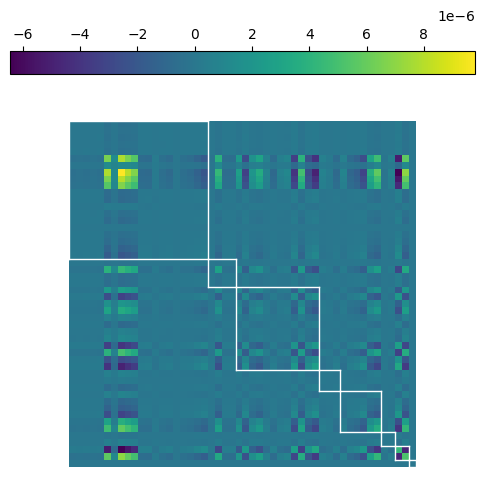
\includegraphics[width=0.43\linewidth]{kfac_pinns_exp/exp04_gramian_contributions/fig/gram_full.png}

  \begin{tabular}{ccc}
    (\textcolor{blue}{forward}, \textcolor{red}{forward})
    &
      (\textcolor{blue}{forward}, \textcolor{red}{gradient})
    &
      (\textcolor{blue}{forward}, \textcolor{red}{Hessian})
    \\
    
\includegraphics[width=0.22\linewidth]{kfac_pinns_exp/exp04_gramian_contributions/fig/gram_output_output.png}
    &
      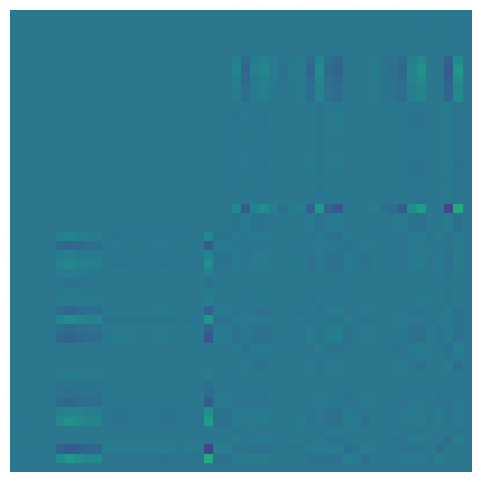
\includegraphics[width=0.22\linewidth]{kfac_pinns_exp/exp04_gramian_contributions/fig/gram_output_grad_input.png}
    &
      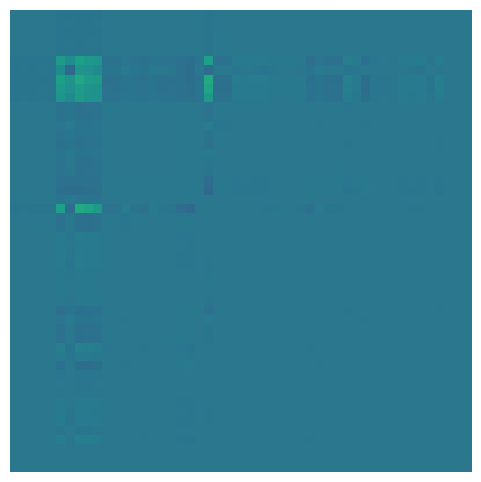
\includegraphics[width=0.22\linewidth]{kfac_pinns_exp/exp04_gramian_contributions/fig/gram_output_hess_input.png}
    \\
    (\textcolor{blue}{gradient}, \textcolor{red}{forward})
    &
      (\textcolor{blue}{gradient}, \textcolor{red}{gradient})
    &
      (\textcolor{blue}{gradient}, \textcolor{red}{Hessian})
    \\
    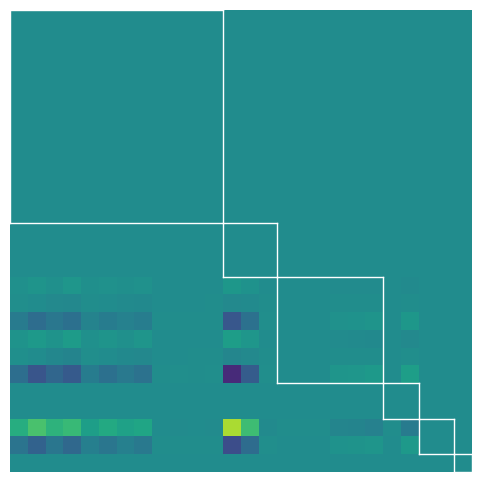
\includegraphics[width=0.22\linewidth]{kfac_pinns_exp/exp04_gramian_contributions/fig/gram_grad_input_output.png}
    &
      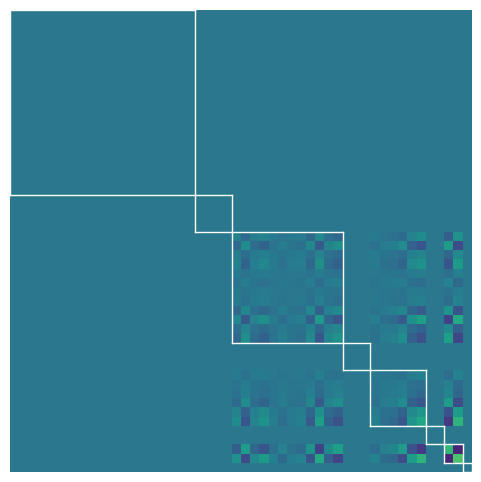
\includegraphics[width=0.22\linewidth]{kfac_pinns_exp/exp04_gramian_contributions/fig/gram_grad_input_grad_input.png}
    &
      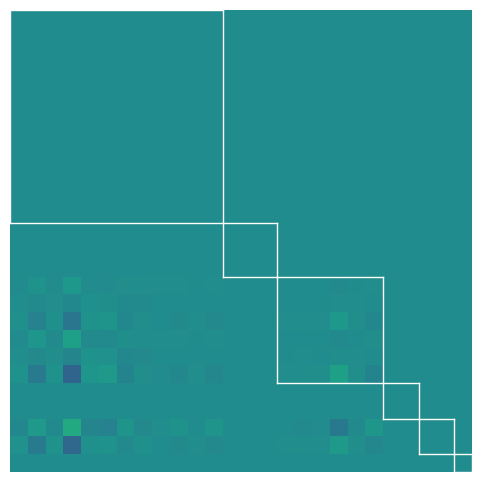
\includegraphics[width=0.22\linewidth]{kfac_pinns_exp/exp04_gramian_contributions/fig/gram_grad_input_hess_input.png}
    \\
    (\textcolor{blue}{Hessian}, \textcolor{red}{forward})
    &
      (\textcolor{blue}{Hessian}, \textcolor{red}{gradient})
    &
      (\textcolor{blue}{Hessian}, \textcolor{red}{Hessian})
    \\
    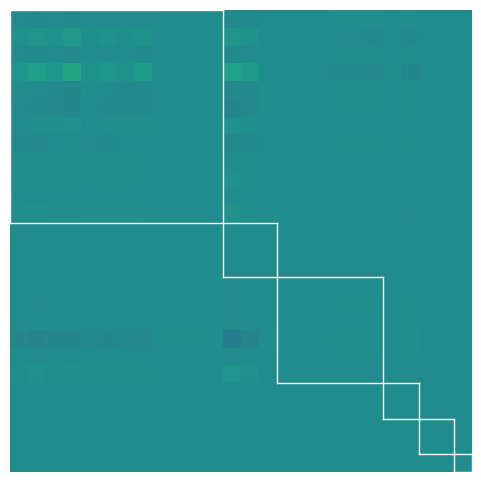
\includegraphics[width=0.22\linewidth]{kfac_pinns_exp/exp04_gramian_contributions/fig/gram_hess_input_output.png}
    &
      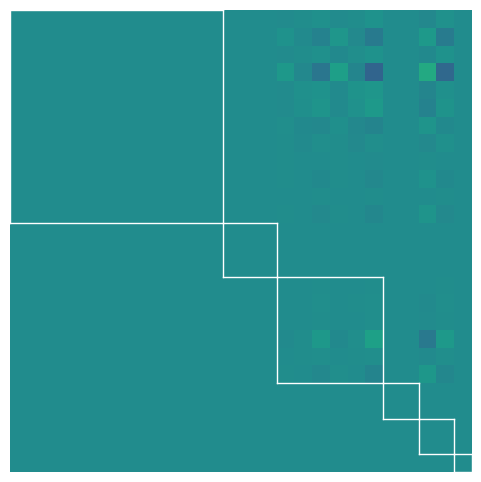
\includegraphics[width=0.22\linewidth]{kfac_pinns_exp/exp04_gramian_contributions/fig/gram_hess_input_grad_input.png}
    &
      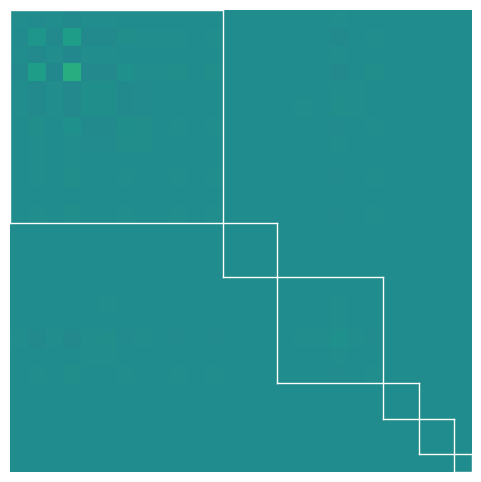
\includegraphics[width=0.22\linewidth]{kfac_pinns_exp/exp04_gramian_contributions/fig/gram_hess_input_hess_input.png}
  \end{tabular}
  \caption{Contributions $\mG_{\Omega,\textcolor{blue}{\bullet}, \textcolor{red}{\bullet}}$ to the Laplacian's Gramian $\mG_{\Omega}$ from different children in the computation graph on a synthetic toy problem.
    We use a $4 \to 3 \to 2 \to 1$ sigmoid-activated MLP and 10 randomly generated inputs. The contributions are highlighted as in \Cref{eq:fisher}.}\label{fig:gramian-contribution-children}
\end{figure}
%%% Local Variables:
%%% mode: latex
%%% TeX-master: "../main"
%%% End:


\paragraph{Computing $\jac_{\mW^{(i)}}\bullet$}
Let us first compute the Jacobians $\jac_{\mW^{(i)}}\bullet$ in \Cref{eq:laplacian-gradient}.
The Jacobian of the linear layer's forward pass is
\begin{subequations}\label{eq:fisher-jacobians}
  \begin{align}
    \jac_{\mW}\left( \mW \vx \right) = \vx^{\top} \otimes \mI\,.
  \end{align}
  The Jacobian from the gradient backpropagation is
  \begin{align}
    \jac_{\mW}\left( \mW^{\top} \vx \right) = \mI \otimes \vx^{\top}\,,
  \end{align}
  and the Jacobian from the Hessian backpropagation is
  \begin{align}\label{subeq:fisher-jacobians-hbp}
    \jac_{\mW}\left( \mW^{\top} \mX \mW \right)
    =
    \mI \otimes \mW^{\top}\mX
    +
    \mK \left(
    \mI
    \otimes
    \mW^{\top}\mX^{\top}
    \right)\,,
  \end{align}
\end{subequations}
where $\mK \in \sR^{\dim(\mZ) \times \dim(\mZ)}$ (denoting $\mZ := \mW^{\top}\mX \mW$) is a permutation matrix that, when multiplied onto a vector whose basis corresponds to that of the flattened output $\mZ$, modifies the order from first-varies-fastest to last-varies-fastest, i.e.
\begin{equation*}
  \mK \flatten(\mZ) = \flatten(\mZ^{\top})\,.
\end{equation*}
Re-introducing the layer indices, the expressions in \Cref{eq:spatialDerivatives} become
\begin{align}
  \begin{split}
    \jac_{\mW^{(i)}}\vz^{(i)}
    &=
      {\vz^{(i-1)}}^\top\otimes \mI
    \\
    \jac_{\mW^{(i)}}\grad{\vz^{(i-1)}}u\,,
    &=
      \mI\otimes
      \grad{\vz^{(i)}}u
    \\
    \jac_{\mW^{(i)}}\gradsquared{\vz^{(i-1)}}u\,,
    &=
      \mI \otimes
      \left[
      {\mW^{(i)}}^{\top}
      \left(
      \gradsquared{\vz^{(i)}}u
      \right)
      \right]
      +
      \mK
      \left(
      \mI \otimes
      \left[
      {\mW^{(i)}}^{\top}
      \left(
      \gradsquared{\vz^{(i)}}u
      \right)^{\top}
      \right]
      \right)\,.
  \end{split}
\end{align}
We will now use symmetries in the objects used during Hessian backpropagation to simplify this further.
At a first glance, it looks like the Gramian consists of 16 terms, as there are 4 summands from the Jacobians in \Cref{eq:fisher-jacobians}.
However, we can simplify into 9 terms:

First, $\gradsquared{\vz^{(i)}}u$ is symmetric, that is
\begin{align*}
  \jac_{\mW^{(i)}}\left( {\mW^{(i)}}^{\top} \left( \gradsquared{\vz^{(i)}}u  \right)\mW^{(i)} \right)
  &=
    \mI \otimes
    \left[
    {\mW^{(i)}}^{\top} \left( \gradsquared{\vz^{(i)}}u  \right)
    \right]
    +
    \mK
    \left(
    \mI \otimes
    \left[
    {\mW^{(i)}}^{\top}
    \left(
    \gradsquared{\vz^{(i)}}u
    \right)
    \right]
    \right)\,,
    \shortintertext{and the transposed Jacobian is}
  &\mI \otimes
    \left[
    \left( \gradsquared{\vz^{(i)}}u  \right) \mW^{(i)}
    \right]
    +
    \left(
    \mI \otimes
    \left[
    \left(
    \gradsquared{\vz^{(i)}}u
    \right)
    \mW^{(i)}
    \right]
    \right)
    \mK^{\top}\,.
\end{align*}
Second, we multiply the transpose Jacobian onto $\grad{\gradsquared{\vz^{(i-1)}}u}\Delta u$, which inherits symmetry from the Hessian, $[\grad{\gradsquared{\vz^{(i-1)}}u}\Delta u]_{j,k} = [\grad{\gradsquared{\vz^{(i-1)}}u}\Delta u]_{k,j}$.
Due to this symmetry, the action of $\mK$ (or $\mK^{\top}$) does not alter it,
\begin{align*}
  \mK^{\top}\left( \grad{\gradsquared{\vz^{(i-1)}}u}\Delta u \right) = \grad{\gradsquared{\vz^{(i-1)}}u}\Delta u\,.
\end{align*}
In other words, it does not matter how we flatten (first- or last-varies-fastest).
This simplifies the VJP (last line in \Cref{eq:fisher}) to
\begin{align*}
  \left(
  \mI \otimes
  \left[
  \left( \gradsquared{\vz^{(i)}}u  \right) \mW^{(i)}
  \right]
  \right)
  \grad{\gradsquared{\vz^{(i-1)}}u}\Delta u
  +
  \left(
  \mI \otimes
  \left[
  \left(
  \gradsquared{\vz^{(i)}}u
  \right)
  \mW^{(i)}
  \right]
  \right)
  \mK^{\top}
  \grad{\gradsquared{\vz^{(i-1)}}u}\Delta u
  \\
  =
  2 \left(
  \mI \otimes
  \left[
  \left( \gradsquared{\vz^{(i)}}u  \right) \mW^{(i)}
  \right]
  \right)
  \grad{\gradsquared{\vz^{(i-1)}}u}\Delta u
  \,.
\end{align*}
We can now write down the simplified Jacobian from \Cref{eq:laplacian-gradient}, whose self-outer product forms the Gramian block for a linear layer's weight matrix,
\begin{align}\label{eq:weight-jacobian-simplified}
  \begin{split}
    \jac_{\mW^{(i)}} \Delta u
    &=
      \underbrace{
      \left(
      {\vz^{(i-1)}}^\top\otimes \mI
      \right)^{\top}
      \grad{\vz^{(i)}}\Delta u
      }_{(1)}
    \\
    &\phantom{=}+
      \underbrace{
      \left(
      \mI \otimes \grad{\vz^{(i)}}u
      \right)^{\top}
      \grad{\grad{\vz^{(i-1)}}u}\Delta u
      }_{(2)}
    \\
    &\phantom{=}+
      \underbrace{
      2
      \left(
      \mI \otimes
      \left[
      \left( \gradsquared{\vz^{(i)}}u \right) \mW^{(i)}
      \right]
      \right)
      \grad{\gradsquared{\vz^{(i-1)}}u}\Delta u
      }_{(3)}
      \,,
  \end{split}
\end{align}
where (1) is the contribution from the forward pass, (2) is the contribution from the gradient backpropagation, and (3) is the contribution from the Hessian backpropagation. The Jacobians from \Cref{eq:fisher-jacobians} allow to express the Gramian in terms of Kronecker-structured expressions consisting of 9 terms in total. \Cref{fig:gramian-contribution-children} shows the 6 contributions from different children pairs.

\paragraph{Conclusion} One problem of computing the Laplacian and its Jacobian with backpropagation according to \Cref{eq:weight-jacobian-simplified} is that if we write out the Gramian's block $\mG_{\Omega}^{(i)} = \jac_{\mW^{(i)}} \Delta u (\jac_{\mW^{(i)}} \Delta u)^{\top}$, we obtain 9 terms of different structure.
Defining a single Kronecker product approximation would involve introducing new approximations on top of those employed by \citet{eschenhagen2023kroneckerfactored}.
Therefore, the forward Laplacian, or Taylor-mode, perspective we choose in the main text is advantageous as it allows to define KFAC without introducing new approximations.

\paragraph{Computing $\grad{\textcolor{blue}{\bullet}}\Delta u$}
The terms $\grad{\textcolor{blue}{\bullet}}\Delta u$ are automatically computed when computing the gradient of the loss via backdrop.

%%% Local Variables:
%%% mode: latex
%%% TeX-master: "../main"
%%% End:



%%% Local Variables:
%%% mode: latex
%%% TeX-master: "../main"
%%% End:



\section{Example: Laplacian for a Shallow Network}

Here, we compute the Laplacian for a less general, yet simpler, example: A shallow neural network.

\begin{comment}
  For the one-dimensional shallow case we have
  \[ u_\theta(x) = \sum_{i=1}^m a_i\sigma(b_i x + c_i) + d. \]
  Then
  \[ u_\theta'(x) = \sum_{i=1}^m a_ib_i\sigma'(b_i x + c_i) \]
  and
  \[ u_\theta''(x) = \sum_{i=1}^m a_ib_i^2\sigma''(b_i x + c_i). \]
  The parameter derivative of the Laplacian (i.e., second-order derivative)
  \begin{align*}
    \partial_{a_i}u_\theta''(x) & = b_i^2\sigma''(b_i x + c_i) \\
    \partial_{b_i}u_\theta''(x) & = 2a_ib_i\sigma''(b_i x + c_i) + a_i b_i^2x\sigma^{(3)}(b_i x + c_i) \\
    \partial_{c_i}u_\theta''(x) & = a_i b_i^2\sigma^{(3)}(b_i x + c_i) \\
    \partial_{d}u_\theta''(x) & = 0.
  \end{align*}
  The parameter derivative of the Laplacian (i.e., second-order derivative)
  \begin{align*}
    \partial_{a_i}u_\theta''(x) & = b_i^2\sigma''(b_i x + c_i) \\
    \partial_{b_i}u_\theta''(x) & = 2a_ib_i\sigma''(b_i x + c_i) + a_i b_i^2x\sigma^{(3)}(b_i x + c_i) \\
    \partial_{c_i}u_\theta''(x) & = a_i b_i^2\sigma^{(3)}(b_i x + c_i) \\
    \partial_{d}u_\theta''(x) & = 0.
  \end{align*}
\end{comment}

First, we do the Hessian calculation as explicitly as possible. For this, we consider the easy case of a shallow network with one-dimensional output
\[ u_\theta(x) = \sum_{i=1}^m a_i\sigma(b_i^\top x + c_i) + d. \]
Then
\[ \nabla_x u_\theta(x) = \sum_{i=1}^m a_ib_i\sigma'(b_i x + c_i) \]
or
\[ \partial_{x_j} u_\theta(x) = \sum_{i=1}^m a_i(b_i)_j\sigma'(b_i x + c_i). \]
Consequently, we compute
\[ \partial_{x_k}\partial_{x_j} u_\theta(x) = \sum_{i=1}^m a_i(b_i)_j(b_i)_k\sigma'(b_i x + c_i) \]
which yields the Hessian
\[ \nabla^2_x u_\theta(x) = \sum_{i=1}^m a_i\sigma''(b_i x + c_i) \cdot b_ib_i^\top = \sum_{i=1}^m a_i\sigma''(b_i x + c_i) \cdot  b_i\otimes b_i \]
and the Laplacian is given by
\[ \Delta_x u_\theta(x) = \sum_{i=1}^m a_i\sigma''(b_i x + c_i) \operatorname{tr}(b_ib_i^\top) = \sum_{i=1}^m a_i\sigma''(b_i x + c_i)  \operatorname{tr}(b_i\otimes b_i). \]
The parameter derivatives of the Hessian are given
\begin{align*}
  \partial_{a_i}\nabla_x^2 u_\theta(x) & = \sigma''(b_i x + c_i) b_ib_i^\top \\
  \nabla_{b_i}\nabla_x^2 u_\theta(x) & = a_i\sigma''(b_i x + c_i) (b_i\otimes I+I\otimes b_i) + a_i \sigma^{(3)}(b_i x + c_i) \cdot  (I\otimes x^\top)(b_i\otimes b_i) \quad ?? \\
  % + a_i x\sigma^{(3)}(b_i x + c_i) \cdot b_ib_i^\top \\
     \partial_{c_i}\nabla_x^2 u_\theta(x) & = a_i b_i^2\sigma^{(3)}(b_i x + c_i) \\
     \partial_{d}\nabla_x^2 u_\theta(x) & = 0.
\end{align*}
The parameter derivatives of the Laplacian are given
\begin{align*}
     \partial_{a_i}\Delta_x u_\theta(x) & = \sigma''(b_i x + c_i) \operatorname{tr}(b_ib_i^\top) \\
     \nabla_{b_i}\Delta_x u_\theta(x) & = 2a_i\sigma''(b_i x + c_i) + a_i \sigma^{(3)}(b_i x + c_i) \operatorname{tr}(b_ib_i^\top) \cdot x \\
     \partial_{c_i}\Delta_x u_\theta(x) & = a_i \sigma^{(3)}(b_i x + c_i)\operatorname{tr}(b_ib_i^\top) \\
     \partial_{d}\Delta_x u_\theta(x) & = 0.
\end{align*}


\paragraph{Writing as linear algebra}

Consider a shallow network
\[ u_\theta(x) = W_2\sigma(W_1 x), \]
where $x\in\mathbb R^d$, $W_1\in\mathbb R^{m\times d}, W_2\in\mathbb R^{1\times m}$.

\paragraph{Task: }
Understand the structure, in particular the computational graph of $f_\theta = \Delta u_\theta$.

\paragraph{One dimensional case: }
Assume first that $d=1$.
Then
\[ D_x u_\theta(x) = W_2 \operatorname{diag}(\sigma'(W_1 x)) W_1 \]
and
\[ D^2_x u_\theta(x) = W_2%(W_1^\top\otimes W_2)
  \operatorname{diag}(\operatorname{diag}(\sigma''(W_1 x)) W_1)W_1. % = W_2 \operatorname{diag}\sigma''(W_1 x) W_1^2 = W_2\odot W_1^2 \sigma''(W_1x),
\]
In another form
\[D^2 u_\theta(x) = W_2 \operatorname{diag}(\operatorname{diag}\sigma''(W_1 x) W_1) W_1 = W_2 \operatorname{diag}\sigma''(W_1 x) W_1^2 = W_2\odot W_1^2 \sigma''(W_1x),
\]
where $(W_2\odot W_1^2)_k = (W_2)_k \cdot (W_1)_k^2$.
% where $(W_2\odot W_1^2)_k = (W_2)_k \cdot (W_1)_k^2$.
% The Laplacian is then given as
% \[ f_\theta(x) = \Delta u_\theta(x) = \operatorname{tr}(D_x^2u_\theta(x)) =\operatorname{tr}(W_2 \operatorname{diag}(\operatorname{diag}(\sigma''(W_1 x)) W_1) W_1).  \]
% Differentiation with respect to $W_2$ yields
% \[ \frac{\partial f_\theta(x)}{\partial W_2} = \frac{\partial \Delta u_\theta(x)}{ \partial W_2} =  \]

One can also rewrite the diagonalization operator via a Hadamard product as $\operatorname{diag}(x) = (x\mathds{1}^\top)\odot I$, where $\mathds{1}$ denotes the all one vector, $I$ the identity and $\odot$ the Hadamard (i.e., entrywise) product of two matrices.
Not sure whether this helps though...

\paragraph{Multi-dimensional case}

%%% Local Variables:
%%% mode: latex
%%% TeX-master: "../main"
%%% End:


\end{document}

%%% Local Variables:
%%% mode: latex
%%% TeX-master: t
%%% End:
